\documentclass[a4paper, 12pt]{article}
\usepackage[utf8]{inputenc}

\usepackage{subcaption}
\usepackage{enumitem}
\usepackage{caption}
\usepackage{wrapfig}
\usepackage{graphicx}
\usepackage{mathtext}
\usepackage{amsmath}
\usepackage{amssymb}
\usepackage{amsfonts}
\usepackage{siunitx}
\usepackage{multirow}
\usepackage{rotating}
\usepackage{float}
\usepackage{longtable}
\usepackage{comment}

\usepackage[demo]{graphicx}
\usepackage[T1,T2A]{fontenc}
\usepackage[russian]{babel}

\graphicspath{{images/}}

\title{
    \begin{center}
        Лабораторная работа №1.2.4
    \end{center}
    \begin{center}
        Определение главных моментов инерции твердых тел с помощью крутильных колебаний
    \end{center}
    \begin{center}
        МФТИ, ФЭФМ 1 курс
    \end{center}   
}

\author{Евтушенко Ольга, Б04-306}
\date{01.11.2023}



\begin{document}
    \pagenumbering{gobble}
    \maketitle
    \newpage
    \pagenumbering{arabic}

    \section*{Введение}

    \noindent\textbf{Цель работы:} 
    \begin{enumerate}
        \item измерить периоды крутильных колебаний рамки при различных положениях закрепленного в ней тела; 
        \item проверить теоретическую зависимость между периодами крутильных колебаний тела относительно различных осей; 
        \item определить моменты инерции относительно нескольких осей для каждого тела, по ним найти главные моменты инерции тел и построить эллипсоид инерции.
    \end{enumerate}
    
    \vspace{0.35cm}
    
    \noindent\textbf{В работе используются:} 
    \begin{enumerate}
        \item установка для получения крутильных колебаний (жесткая рамка, имеющая винты для закремления в ней твердых тел, подвешенная на натянутой вертикально проволоке);
        \item набор исследуемых твердых тел;
        \item секундомер.
    \end{enumerate}

    \newpage
    
    \section*{Теоретические сведения}
        Инерциальные свойства твердого тела при вращении определяется не только величиной его массы, но и ее пространственным распределением, которое характеризуется тензором инерции. Тензор инерции может быть представлен в виде симметричной матрицы, определяющейся шестью элементами:
            
        \begin{equation*}
            \hat{I} =
            \begin{Vmatrix}
                I_{xx} & I_{xy} & I_{xz}\\
                I_{yx} & I_{yy} & I_{yz}\\
                I_{zx} & I_{zy} & I_{zz}
            \end{Vmatrix},\;где\;\;\;\;\;
            \begin{aligned}
                & I_{xx} = \int (y^2 + z^2)\, \mathrm{d}m,\\ 
                & I_{xy} = -\int xy\, \mathrm{d}m, \\
                & I_{xz} = -\int xz\, \mathrm{d}m\;и\;т.п.
            \end{aligned}
        \end{equation*}
        Так как $\hat{I}$ -- симметричная матрица, ее можно привести к виду
        \begin{equation*}
            \hat{I} =
            \begin{Vmatrix}
                I_{x} & 0 & 0\\
                0 & I_{y} & 0\\
                0 & 0 & I_{z}
            \end{Vmatrix},
        \end{equation*}
        где $I_x,\;I_y,\;I_z$ -- главные моменты инерции тела. 
        
        Геометрическим образом $\hat{I}$ является эллипсоид, называемый эллипсоидом инерции, уравнение которого в главных осях имеет вид:
        \begin{equation}
            I_xx^2 + I_yy^2 + I_zz^2 = 1.
        \end{equation}
        Эллипсоид инерции жестко связан с телом, для которого построен: координатные оси $Ox,\;Oy,\;Oz$ совпадают с главными осями тела. Если Начало координат $O$ совпадает с центром масс тела, такой эллипсоид инерции называется центральным.

        Зная эллипсоид инерции, можно найти момент инерции тела относительно любой оси, проходящей через центр эллипсоида. Пусть $\vec{r}$ -- радиус-векто вдоль выбранной оси до пересечения с поверхностью эллипсоида. Тогда момент инерции тела относительно этой оси будет:
        \begin{equation}
            I = \frac{1}{r^2}.
        \end{equation}

        Главные оси тела можно определить из его симметрии.

        \newpage

        \begin{figure}[h]
            \begin{center}$
                \begin{array}{cc}
                    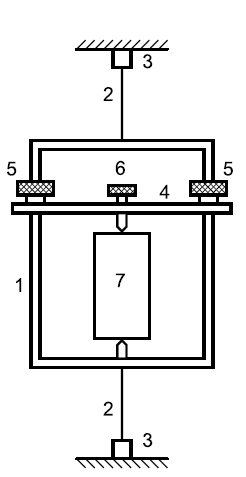
\includegraphics[width=0.3\textwidth]{installation}&
                    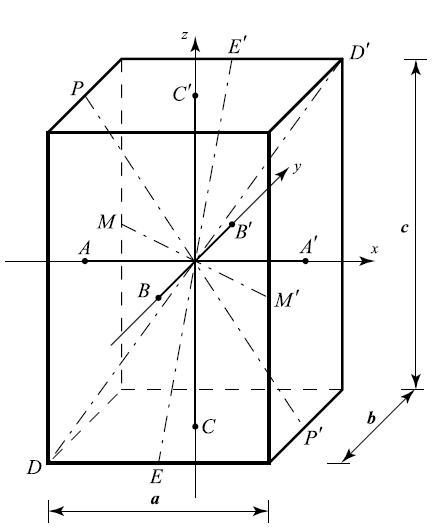
\includegraphics[width=0.49\textwidth]{cube}\\
                    \text{Рис. 1: Схема установки} & 
                    \text{Рис. 2: Оси вращения }\\
                    &\text{прямоугольного параллелепипеда}
                \end{array}$
            \end{center}
        \end{figure}

       % \begin{wrapfigure}{l}{0.3\textwidth}
        %     \centering
        %     \captionsetup{justification=centering}
        %     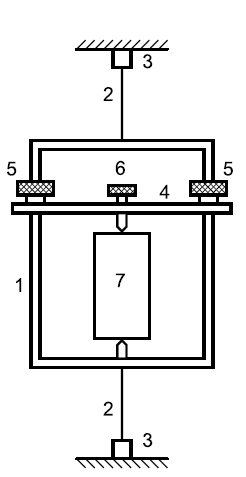
\includegraphics[width=1.0\linewidth]{installation.png}
        %     \caption{Схема установки}
        % \end{wrapfigure}
        
        \vspace{-7mm}
        В данной работе будем использовать устройство для получения крутильных колебаний, изображенное на рис. 1. Рамка 1 жестко соединена с проволокой 2, закрепленной вертикально в специальных зажимах 3, позволяющих сообщить начальне закручивание для возбуждения крутильных колебаний вокруг вертикальной оси. В рамке с помощью планки 4, гаек 5 и винта 6 закрепляется твердое тело 7. На теле имеются специальные выемки, позволяющие его закрепить так, чтобы ось вращения проходила в теле под различнвми углами через центр масс.
        
        Крутильные колебания рамки с телом описываются уравнением
        \vspace{-3mm}
        \begin{equation}
            (I + I_{р})\frac{\mathrm{d}^2\varphi}{\mathrm{d}t^2} = -f\varphi,
        \end{equation}
        где $I\;и\;I_p$ -- моменты инерции тела и рамки относительно оси вращения, $\varphi$ -- угол поворота рамки, меняющийся со временем, $t,\;f$ -- модуль кручения проволоки.

        Тогда период крутильных колебаний рамки с телом определяется формулой
        \begin{equation}
            T = 2\pi\sqrt{\frac{I + I_{р}}{f}}.
        \end{equation}

        На рис. 2 показано, как проходят оси вращения в параллелепипеде. Оси $AA',\;BB'\;и\;CC'$ являются главными. Пусть $I_x,\;I_y,\;I_z$ -- моменты инерции относительно этих осей соответственно. Ось $DD'$, проходящая вродь диагонали параллелепипеда, с главными осями составляет те же углы, что с ребрами $a,\;b\;и\;c$, так как они им параллельны. Косинусы этих углов равны соответственно $a/d,\;b/d\;и\;c/d$, где длина диагонали $d = \sqrt{a^2 + b^2 + c^2}$.

        Момент инерции $I_d$ при вращении относительно диагонали $DD'$ выражается следующим образом:
        \begin{equation}
            I_d = I_x\frac{a^2}{d^2} + I_y\frac{b^2}{d^2} + I_z\frac{c^2}{d^2},
        \end{equation}
        откуда получаем соотношение
        \begin{equation}
            (a^2 + b^2 + c^2)I_d = a^2I_x + b^2I_y + c^2I_z.
        \end{equation}
        Через связь $I\;и\;T$ из (4) получим соотношение между периодами колебаний:
        \begin{equation}
            (a^2 + b^2 + c^2)T_d^2 = a^2T_x^2 + b^2T_y^2 + c^2T_z^2.
        \end{equation}
        
        % \begin{wrapfigure}{r}{0.5\textwidth}
        %     \centering
        %     \captionsetup{justification=centering}
        %     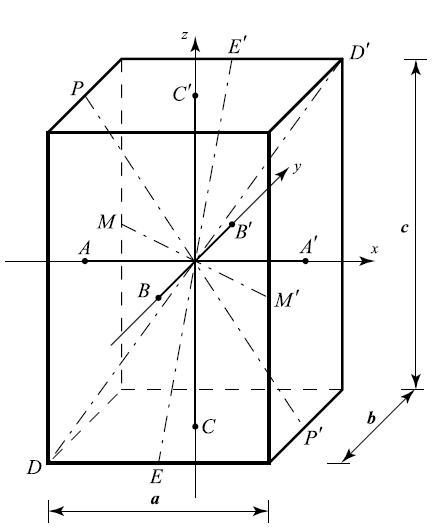
\includegraphics[width=1.0\linewidth]{cube.png}
        %     \caption{Оси вращения прямоугольного параллелепипеда}
        % \end{wrapfigure}

        Экспериментальная проверка соотношения (7) также проверим соотношение (5). Из этой формулы следуют выражения, связывающие периоды колебаний относительно осей $EE',\;MM'\;и\;PP'$:
        \begin{equation}
            (b^2 + c^2)T_E^2 = b^2T_y^2 + c^2T_z^2,
        \end{equation}
        \begin{equation}
            (a^2 + c^2)T_P^2 = a^2T_x^2 + c^2T_z^2,
        \end{equation}
        \begin{equation}
            (a^2 + b^2)T_M^2 = a^2T_x^2 + b^2T_y^2,
        \end{equation}
        которые тоже следует проверить экспериментально.

    \newpage
        
    \section*{Ход работы}
        1. Ознакомимся с установкой для получения крутильных колебаний. Проверим:
        \begin{enumerate}[label=\arabic*)]
            \item хорошо ли натянута проволока,
            \item жестко ли закреплена на ней рамка, 
            \item нормально ли работает устройство для возбуджения крутильных колебаний,
            \item не возникают ли, кроме крутильных колебаний рамки, еще и колебания в вертикальной плоскоти (их не должно быть).
        \end{enumerate}   

        2. Закрепим тело в рамке так, чтобы оно не поворачивалось в ней при вращении конструкции.

        3. Перед каждой серией измерений будем выбирать такую амплитуду крутильных колебаний, чтобы за 15 колебаний амплитуда уменьшалась не более, чем вдвое.
        
        % \vspace{-4mm}
        \begin{figure}[h]
            \begin{center}$
                \begin{array}{cc}
                    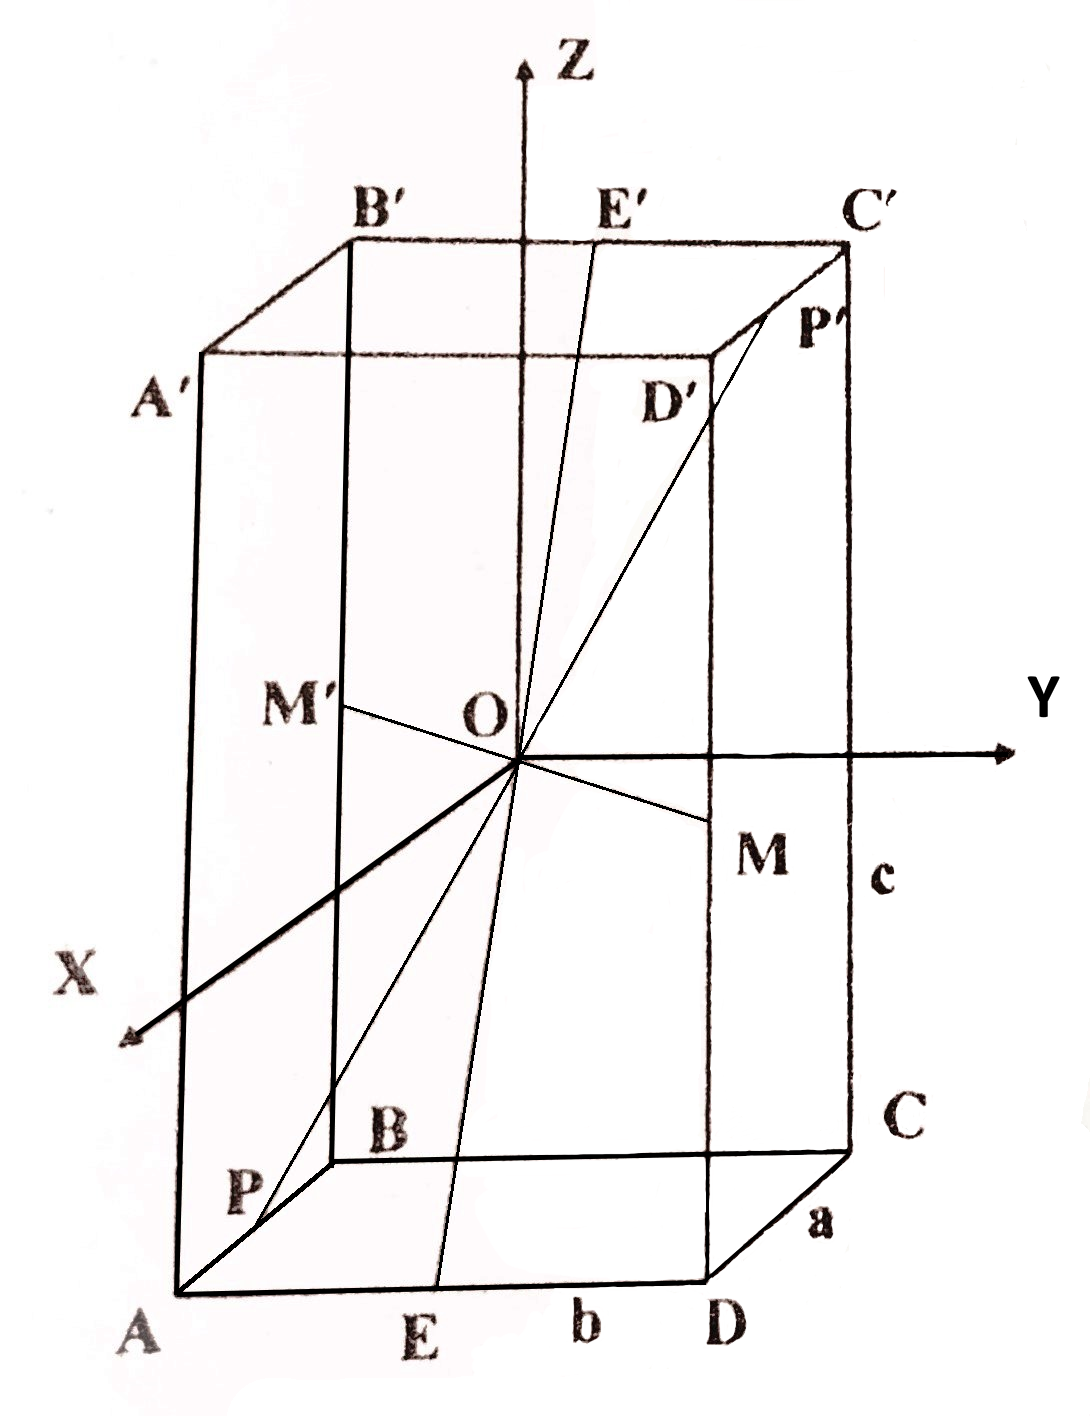
\includegraphics[width=0.3\textwidth]{cube_1}&
                    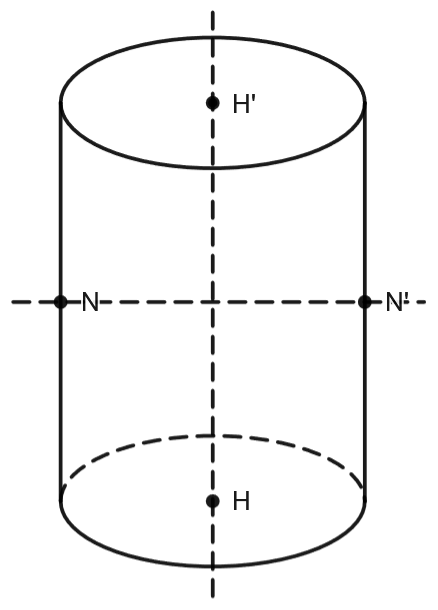
\includegraphics[width=0.27\textwidth]{cylinder-2}\\
                    \text{Рис. 3: Оси параллелепипеда} & 
                    \text{Рис. 4: Оси цилиндра}
                \end{array}$
            \end{center}
        \end{figure}
        \vspace{-6mm}
        
        4. Для рамки и каждого изучаемого тела проведем серии экспериментов (по 3 раза, положения тел различны относительно осей) по определению периода колебаний $n = 15$ колебаний для каждой из осей. У рамки (без дополнительных тел) только одна ось, проходящая вдоль вертикальной оси $Oz$; у каждого из цилиндров по две -- $HH'$, проходящая через ось симметрии, и $NN'$, проходящая через центр $HH'$ параллельно диаметру оснований (рис. 4); у параллелепипеда 7 -- вдоль осей $Ox,\;Oy\;и\;Oz$, $MM',\;EE',\;PP'\;и\;AC'$ (рис. 3); у куба в силу его симметрии достаточно рассмотреть только 3 -- $Ox,\;MM'\;и\;AC'$ (аналогично конфигурации на рис. 3). Результаты занесем в таблицы 1-5.

        \begin{table}
            \centering
            \caption{Периоды колебаний рамки}
            \begin{tabular}{|c|cc|}
                \hline
                Ось & \multicolumn{2}{c|}{$Oz$} \\
                \hline
                № измерения & \multicolumn{1}{l|}{$\tau$, c} & $T$, c \\
                \hline
                1 & \multicolumn{1}{c|}{67,62} & 4,51 \\
                \hline
                2 & \multicolumn{1}{c|}{66,84} & 4,46 \\
                \hline
                3 & \multicolumn{1}{c|}{67,26} & 4,48 \\
                \hline
                Среднее & \multicolumn{1}{c|}{67,24} & 4,48 \\
                \hline
            \end{tabular}
        \end{table}

        \begin{table}
            \centering
            \caption{Периоды колебаний цилиндров}
            \begin{tabular}{|c|cccc|cccc|}
                \hline
                & \multicolumn{4}{c|}{Низкий цилиндр}
                & \multicolumn{4}{c|}{Высокий цилиндр} \\
                \hline
                Ось 
                & \multicolumn{2}{c|}{$HH'$} 
                & \multicolumn{2}{c|}{$NN'$} 
                & \multicolumn{2}{c|}{$HH'$} 
                & \multicolumn{2}{c|}{$NN'$} \\
                \hline
                № измерения 
                & \multicolumn{1}{c|}{$\tau$, c} 
                & \multicolumn{1}{c|}{$T$, c} 
                & \multicolumn{1}{c|}{$\tau$, c} 
                & $T$, c 
                & \multicolumn{1}{c|}{$\tau$, c} 
                & \multicolumn{1}{c|}{$T$, c} 
                & \multicolumn{1}{c|}{$\tau$, c} 
                & $T$, c \\
                \hline
                1 
                & \multicolumn{1}{c|}{90,44} 
                & \multicolumn{1}{c|}{6,03} 
                & \multicolumn{1}{c|}{80,11} 
                & 5,34   
                & \multicolumn{1}{c|}{84,39} 
                & \multicolumn{1}{c|}{5,63} 
                & \multicolumn{1}{c|}{79,63}     
                & 5,31 \\
                \hline
                2           
                & \multicolumn{1}{c|}{90,53}     
                & \multicolumn{1}{c|}{6,04}   
                & \multicolumn{1}{c|}{80,35}     
                & 5,36   
                & \multicolumn{1}{c|}{83,60}     
                & \multicolumn{1}{c|}{5,57}   
                & \multicolumn{1}{c|}{79,42}     
                & 5,29 \\
                \hline
                3           
                & \multicolumn{1}{c|}{90,02}     
                & \multicolumn{1}{c|}{6,00}   
                & \multicolumn{1}{c|}{80,06}     
                & 5,34   
                & \multicolumn{1}{c|}{85,08}     
                & \multicolumn{1}{c|}{5,67}   
                & \multicolumn{1}{c|}{79,38}     
                & 5,29 \\
                \hline
                Среднее     
                & \multicolumn{1}{c|}{90,33}     
                & \multicolumn{1}{c|}{6,02}   
                & \multicolumn{1}{c|}{80,17}     
                & 5,34   
                & \multicolumn{1}{c|}{84,36}     
                & \multicolumn{1}{c|}{5,62}   
                & \multicolumn{1}{c|}{79,48}     
                & 5,30 \\
                \hline
            \end{tabular}
        \end{table}

        \begin{table}
            \centering
            \caption{Периоды колебаний параллелепипеда}
            \begin{tabular}{|c|cc|cc|cc|cc|}
                \hline
                Ось
                & \multicolumn{2}{c|}{$Ox$}
                & \multicolumn{2}{c|}{$Oy$}
                & \multicolumn{2}{c|}{$Oz$}
                & \multicolumn{2}{c|}{$MM'$}
                \\
                \hline
                № измерения
                & \multicolumn{1}{c|}{$\tau$, c} & $T$, c
                & \multicolumn{1}{c|}{$\tau$, c} & $T$, c
                & \multicolumn{1}{c|}{$\tau$, c} & $T$, c
                & \multicolumn{1}{c|}{$\tau$, c} & $T$, c \\
                \hline
                1
                & \multicolumn{1}{c|}{104,93} & 7,00
                & \multicolumn{1}{c|}{97,97} & 6,53
                & \multicolumn{1}{c|}{84,80} & 5,65
                & \multicolumn{1}{c|}{99,92} & 6,66 \\
                \hline
                2
                & \multicolumn{1}{c|}{105,41} & 7,03
                & \multicolumn{1}{c|}{97,92} & 6,53
                & \multicolumn{1}{c|}{84,58} & 5,64
                & \multicolumn{1}{c|}{93,55} & 6,24 \\
                \hline
                3
                & \multicolumn{1}{c|}{105,25} & 7,02
                & \multicolumn{1}{c|}{99,00} & 6,60
                & \multicolumn{1}{c|}{84,75} & 5,65
                & \multicolumn{1}{c|}{99,85} & 6,66 \\
                \hline
                Среднее
                & \multicolumn{1}{c|}{105,20} & 7,01
                & \multicolumn{1}{c|}{98,30} & 6,55
                & \multicolumn{1}{c|}{84,71} & 5,65
                & \multicolumn{1}{c|}{97,77} & 6,52 \\
                \hline
            \end{tabular}
        \end{table}

        \begin{table}
            \centering
            \caption{Периоды колебаний параллелепипеда}
            \begin{tabular}{|c|cc|cc|cc|}
                \hline
                Ось
                & \multicolumn{2}{c|}{$EE'$}
                & \multicolumn{2}{c|}{$PP'$}
                & \multicolumn{2}{c|}{$AC'$}
                \\
                \hline
                № измерения
                & \multicolumn{1}{c|}{$\tau$, c} & $T$, c
                & \multicolumn{1}{c|}{$\tau$, c} & $T$, c
                & \multicolumn{1}{c|}{$\tau$, c} & $T$, c \\
                \hline
                1
                & \multicolumn{1}{c|}{87,15} & 5,81
                & \multicolumn{1}{c|}{89,58} & 5,97
                & \multicolumn{1}{c|}{90,52} & 6,03 \\
                \hline
                2
                & \multicolumn{1}{c|}{87,03} & 5,80
                & \multicolumn{1}{c|}{89,61} & 5,97
                & \multicolumn{1}{c|}{90,88} & 6,06 \\
                \hline
                3
                & \multicolumn{1}{c|}{87,25} & 5,82
                & \multicolumn{1}{c|}{89,63} & 5,98
                & \multicolumn{1}{c|}{90,89} & 6,06 \\
                \hline
                Среднее
                & \multicolumn{1}{c|}{87,14} & 5,81
                & \multicolumn{1}{c|}{89,61} & 5,97
                & \multicolumn{1}{c|}{90,76} & 6,05 \\
                \hline
            \end{tabular}
        \end{table}

        \begin{table}
            \centering
            \caption{Периоды колебаний куба}
            \begin{tabular}{|c|cc|cc|cc|}
                \hline
                Ось
                & \multicolumn{2}{c|}{$Ox$}
                & \multicolumn{2}{c|}{$MM'$}
                & \multicolumn{2}{c|}{$AC'$}
                \\
                \hline
                № измерения 
                & \multicolumn{1}{c|}{$\tau$, c} 
                & \multicolumn{1}{c|}{$T$, c} 
                & \multicolumn{1}{c|}{$\tau$, c} 
                & \multicolumn{1}{c|}{$T$, c} 
                & \multicolumn{1}{c|}{$\tau$, c} 
                & \multicolumn{1}{c|}{$T$, c} \\
                \hline
                1
                & \multicolumn{1}{l|}{80,20} & 5,35
                & \multicolumn{1}{l|}{80,20} & 5,35
                & \multicolumn{1}{l|}{80,30} & 5,35
                \\
                \hline
                2
                & \multicolumn{1}{l|}{80,52} & 5,37
                & \multicolumn{1}{l|}{80,32} & 5,35
                & \multicolumn{1}{l|}{80,80} & 5,39
                \\
                \hline
                3
                & \multicolumn{1}{l|}{80,10} & 5,34
                & \multicolumn{1}{l|}{80,51} & 5,37
                & \multicolumn{1}{l|}{80,51} & 5,37
                \\
                \hline
                Среднее
                & \multicolumn{1}{l|}{80,27} & 5,35
                & \multicolumn{1}{l|}{80,34} & 5,36
                & \multicolumn{1}{l|}{80,54} & 5,37
                \\
                \hline
            \end{tabular}
        \end{table}

        5. Штангенциркулем измерим геометрические размеры тел, определим длины диагоналей, найдем погрешности. Результаты занесем в таблицы 6 - 7.

        \vspace{-8mm}
        \begin{equation*}
            \begin{aligned}
                 \sigma_{x^2} = 2x\sigma_{x};\\ 
                 \sigma_{\sqrt{x}} = \frac{\sigma_{x}}{2\sqrt{x}};\\
                 \implies 
                 \sigma_{\sqrt{x^2+y^2}} = 
                 \frac{\sigma_{x^2+y^2}}{2\sqrt{x^2+y^2}} = 
                 \frac{\sigma_{x^2}+\sigma_{y^2}}{2\sqrt{x^2+y^2}} =
                 \frac{2x\sigma_{x}+2y\sigma_{y}}{2\sqrt{x^2+y^2}} =
                 \frac{x\sigma_{x}+y\sigma_{y}}{\sqrt{x^2+y^2}};\\
                 \implies \sigma_{\sqrt{x^2+y^2+z^2}} =
                 \frac{x\sigma_{x}+y\sigma_{y}+z\sigma_{z}}{\sqrt{x^2+y^2+z^2}}.
            \end{aligned}
        \end{equation*}

        % \vspace{-6mm}
        \begin{table}[h]
            \centering
            \caption{Геометрические размеры куба и параллелепипеда}
            % \vspace{-3mm}
            \begin{tabular}{|c|c|c|c|c|}
                \hline
                $l$ & Куб & Параллелепипед & $\sigma_{l,\;куб}$, см & $\sigma_{l,\;пар}$, см \\
                \hline
                $a$, cм & 9,24 & 5,04 & 0,005 & 0,005 \\
                \hline
                $b$, cм & 9,26 & 10,01 & 0,005 & 0,005 \\
                \hline
                $c$, cм & 9,27 & 15,00 & 0,005 & 0,005 \\
                \hline
                $MM' = \sqrt{a^2+b^2}$, см & 13,08 & 11,21 & 0,007 & 0,007 \\
                \hline
                $PP' = \sqrt{b^2+c^2}$, см & 13,10 & 18,03 & 0,007 & 0,007 \\
                \hline
                $EE' = \sqrt{a^2+c^2}$, см & 13,09 & 15,82 & 0,007 & 0,006 \\
                \hline
                $AC' = \sqrt{a^2+b^2+c^2}$, см & 16,03 & 18,72 & 0,009 & 0,008 \\
                \hline
            \end{tabular}
        \end{table}
        
        % \vspace{-8mm}
        \begin{table}[h]
            \centering
            \caption{Геометрические размеры цилиндров}
            \vspace{-3mm}
            \begin{tabular}{|c|c|c|c|}
                \hline
                $l$ & Низкий цилиндр & Высокий цилиндр & $\sigma_l$, см \\
                \hline
                $h$, см & 1,19 & 4,9 & 0,005 \\
                \hline
                $d$, см & 12,45 & 8,8 & 0,005 \\
                \hline
            \end{tabular}
        \end{table}

        Измерим массы, их погрешность $\sigma_m = 0,3\;c$. Занесем результаты в таблицу 8.
        
        % \vspace{-8mm}
        \begin{table}[H]
            \centering
            \caption{Массы тел и их обозначение}
            \vspace{-3mm}
            \begin{tabular}{|c|c|c|}
                \hline
                Тело & Обозначение & $m$, г \\
                \hline
                Низкий цилиндр & $m_{нц}$ & 1569,5 \\
                \hline
                Высокий цилиндр & $m_{вц}$ & 2263,8 \\
                \hline
                Куб & $m_{к}$ & 1088,4 \\
                \hline
                Параллелепипед & $m_{п}$ & 2082,8 \\
                \hline
            \end{tabular}
        \end{table}

        Вычислим главные моменты инерции тел относительно каждой из выбранных осей. Все рассматриваемые дальше тела будем считать однородными.

        \subsection*{Момент инерции цилиндра}

        \textbf{а) Относительно оси $\boldsymbol{HH'}$.}

        Чтобы подсчитать момент инерции тонкого диска массы $m$ и радиуса $R$ относительно оси, проходящей через его центр перпендикулярно плоскости диска, разобьем диск на тонкие диски радиуса $dr$. Для каждого из них момент инерции равен $I' = r^2dm$ (так как все точечные массы равноудалены от оси), где $r$ -- расстояние от оси до кольца. Тогда момент инерции всего диска равен
        
        \begin{equation*}
            I_{диск} = \int r^2dm = \int\limits_0^Rr^22\pi rdr \cdot \frac{m}{\pi R^2} = \frac{2m}{R^2} \int\limits_0^R r^3dr = \frac{mR^2}{2}.
        \end{equation*}

        Чтобы найти момент инерции цилиндра массы $m$, радиуса $R$, диаметра $D = 2R$ и высотой $H$ относительно оси $HH'$, разобьем его на тонкие диски высотой $dh$ массы $dm = \frac{m}{H}dh$ вдоль этой оси:
        \vspace{-6mm}
        \begin{equation*}
            \begin{aligned}
                I_{диска} = \frac{dmR^2}{2} = \frac{mR^2}{2H}dh; \\
                \implies I_{HH'} = \int\limits_0^H \frac{mR^2}{2H}dh = \frac{mR^2}{2H}\int\limits_0^Hdh = \frac{mR^2}{2H} \cdot H = \frac{mR^2}{2} = \frac{mD^2}{8}, \\
                \implies \sigma_{I_{HH'}} = \sqrt{\left(\frac{D^2}{8}\right)^2\sigma_m^2 + \left(\frac{m}{8}\cdot2D\right)^2\sigma_D^2} = \frac{D}{8}\sqrt{D^2\sigma_m^2+4m^2\sigma_D^2},
            \end{aligned}
        \end{equation*}
        т.е. момент инерции не зависит от высоты цилиндра.

        \textbf{б) Относительно оси $\boldsymbol{NN'}$.}

        Рассмотрим момент инерции $I_{x}$ тонкого диска радиуса $R$ массы $m$ относительно оси $Ox$, проходящей через его центр вдоль плоскости диска. Пусть ось $Oy$ лежит в этой же плоскости, а $Oz$ -- перпендикулярна. Так как диск -- плоская фигура, то момент инерции относительно точки $\theta = I_z$. В силу симметрии диска относительно $Oz\;I_x = I_y$. Из формулы момента инерции относительно точки получим:
        \begin{equation*}
            2\theta = I_x + I_y + I_z \iff 2I_z = 2I_x + I_z \iff I_x = \frac{I_z}{2} = \frac{mR^2}{4}.
        \end{equation*}

        Чтобы найти момент инерции цилиндра радиуса $R$ массы $m$ высоты $H$ относительно оси $Ox'$ ($NN'$), разрежем его на тонкие диски, диаметры которых являются скрещивающимися к оси $Ox'$. Рассмотрим диск массы $dm = \frac{m}{H}dh$ на расстоянии $h$ от $Ox'$. По теореме Гюйгенса-Штейнера его момент инерции относительно $Ox'$ равен $I'(h) = \frac{dmR^2}{4} + dmh^2$, так как $\frac{dmR^2}{4}$ -- момент инерции этого диска относительно оси, проходящей через его центр масс относительно оси, параллельной $Ox'$, а $h$ -- расстояние от $Ox'$ до центра масс диска. Тогда момент инерции цилиндра относительно $NN'$ равен:
        \begin{equation*}
            \begin{aligned}
            I_{NN'} & = \int \left(\frac{dmR^2}{4} + dmh^2\right) =
            \int\limits_{-H/2}^{H/2} \left(\frac{mR^2}{4H} + \frac{mh^2}{H}\right)dh = \\
            & = \frac{mR^2}{4H}\int\limits_{-H/2}^{H/2} dh\;+\;\frac{m}{H}\int\limits_{-H/2}^{H/2} h^2dh\;=\;
            \frac{mR^2}{4H}H + \frac{m}{H}\left(\frac{H^3}{3 \cdot 8} - \frac{-H^3}{3 \cdot 8}\right) = \\
            & = \frac{mR^2}{4} + \frac{mH^2}{12} = \frac{mD^2}{16} + \frac{mH^2}{12}; \\
            \end{aligned}
        \end{equation*}
        \begin{equation*}
            \begin{aligned}
            \sigma_{I_{NN'}} & = 
            \sqrt{\left(\frac{D^2}{16}\right)^2\sigma_m^2 + \left(\frac{m}{16}\cdot2D\right)^2\sigma_D^2} +
            \sqrt{\left(\frac{H^2}{12}\right)^2\sigma_m^2 + \left(\frac{m}{12}\cdot2D\right)^2\sigma_H^2} = \\
            & = \frac{D}{16}\sqrt{D^2\sigma_m^2+4m^2\sigma_D^2} +
            \frac{H}{12}\sqrt{H^2\sigma_m^2+4m^2\sigma_H^2}.
            \end{aligned}
        \end{equation*}

        \subsection*{Момент инерции параллелепипеда}

        \textbf{а) Относительно оси, параллельной одному из ребер, проходящей через центр масс.}

        Пусть ось $Oz$ параллельна ребру $c$, $Ox$ -- $a$, $Oy$ -- $b$, и все оси проходят через центр масс параллелепипеда.

        Рассмотрим тонкий стержень длины $l$ и массы $m$, перпендикулярный оси $Oz$, проходящей через его центр масс. Пусть ось $Oz'$ паралллельна $Oz$, но проходит через один из концов стержня. Рассмотрим его маленький участок на расстоянии $r$ от оси $Oz'$ массы $dm = \frac{m}{l}dr$. Тогда момент инерции стержня относительно оси $Oz'$ равен:
        \begin{equation*}
            I_{стержень}' = \int r^2dm = \int\limits_0^lr^2\frac{m}{l}dr = \frac{m}{l}\frac{l^3}{3} = \frac{ml^2}{3}.
        \end{equation*}

        \begin{wrapfigure}{l}{0.4\textwidth}
            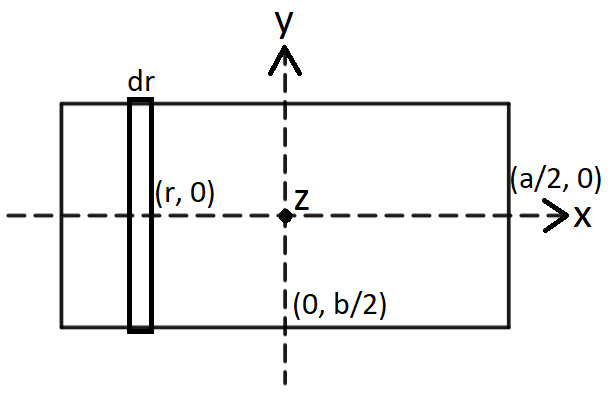
\includegraphics[width=1.0\linewidth]{cubes_IxIy_2}
        \end{wrapfigure}
        По теореме Гюйгенса-Штейнера момент инерции стержня относительно оси $Oz$ равен $I_{стержень} = \frac{ml^2}{3} + m(l/2)^2 = \frac{ml^2}{12}$.
        
        Рассчитаем момент инерции тонкой прямоугольной пластинки, через центр которой проходит ось $Oz$ перпендикулярно плоскости пластинки. Для этого разделим ее на тонкие стержни шириной $dr$, массы $dm = \frac{m}{a}dr$ и длины $b$ вдоль оси $Oy$. 
        
        Тогда искомый инерции равен:
        
        \begin{equation*}
            \begin{aligned}
            I_{пласт, z} & = \int \left(\frac{dmb^2}{12} + dmr^2 \right) =
            \int\limits_{-a/2}^{a/2} \left(\frac{mb^2}{12a} + \frac{mr^2}{a} \right)dr = \\
            & = \frac{mb^2}{12a} \int\limits_{-a/2}^{a/2} dr + \frac{m}{a}\int\limits_{-a/2}^{a/2} r^2dr =
            \frac{mb^2}{12a}a + \frac{m}{a}\left(\frac{a^3}{3 \cdot 8} - \frac{-a^3}{3 \cdot 8} \right) = \\
            & = \frac{m}{12}(a^2 + b^2).
            \end{aligned}
        \end{equation*}

        Чтобы получить момент инерции для параллелепипеда, разделим его на тонкие прямоугольные пластины массы $dm = \frac{m}{c}dr$ вдоль оси $Oz$ на расстоянии $r$ от нее. Тогда искомый инерции имеет вид:
        \begin{equation*}
            \begin{aligned}
            I_{z} & = \int \left(\frac{dm}{12}(a^2+b^2)\right) =\int\limits_{-c/2}^{c/2} \left(\frac{m}{12c}(a^2+b^2)\right)dr = \frac{m}{12}(a^2 + b^2);\\
            & \implies \sigma_{I_{z}} = \frac{\sqrt{a^2+b^2}}{12}\sqrt{(a^2+b^2)\sigma_m^2 + 4m^2\sigma_{\sqrt{a^2+b^2}}^2};
            \end{aligned}
        \end{equation*}
        т.е. он не зависит от длины стороны, вдоль которой направлена ось. 

        Данные для $\sigma_{\sqrt{a^2+b^2}}$ и подобных будем брать из таблицы 6.
        
        Для осей $Ox\;и\;Oy$ моменты инерции определяются аналогично.
        
        \newpage

        \textbf{б) Относительно оси, проходящей через центр масс и соединяющей середины противоположных ребер.}

        Рассмотрим параллелепипед из случая (а). Проведем через его центр масс ось $Oq$, проходящую через середины противоположных ребер длины $b$ ($EE'$ на рис. 3). 

        Из теории раздела II лабораторного практикума имеем формулу (2.53):
        
        \begin{equation*}
            I_q = I_x\cos^2{\alpha} + I_y\cos^2{\beta} + I_z\cos^2{\gamma},
        \end{equation*}
        \begin{equation*}
            где\;\alpha = \angle (Oq, Ox),\;\;\;\beta = \angle (Oq, Oy)\;\;\;и\;\;\;\gamma = \angle (Oq, Oz),
        \end{equation*}
        \begin{equation*}
            т.е:\;\;
            \cos{\alpha} = \frac{a}{\sqrt{a^2+c^2}},
            \;\;\;
            \cos{\beta} = 0,
            \;\;\;
            \cos{\gamma} = \frac{c}{\sqrt{a^2+c^2}};
        \end{equation*}
        \begin{equation*}
            \implies I_q = I_x\frac{a^2}{a^2+c^2} + I_y\cdot 0 + I_z\frac{c^2}{a^2+c^2} = I_x\frac{a^2}{a^2+c^2} + I_z\frac{c^2}{a^2+c^2};
        \end{equation*}

        Будем считать $\sqrt{a^2 + c^2}$ за отдельную переменную.
        \begin{equation*}
            \begin{aligned}
            \implies \sigma_{I_q}^2 & = 
            \left(\frac{a^2}{a^2+c^2}\right)^2\sigma_{I_x}^2 + 
            \left(\frac{c^2}{a^2+c^2}\right)^2\sigma_{I_z}^2 + 
            \left(\frac{2I_xa}{a^2+c^2}\right)^2\sigma_{a}^2 + \\
            & + \left(\frac{2I_zc}{a^2+c^2}\right)^2\sigma_{c}^2 +
            4\left(\frac{I_xa^2+I_zc^2}{(a^2+c^2)^{3/2}}\right)^2\sigma_{\sqrt{a^2+c^2}}^2.
            \end{aligned}
        \end{equation*}
        Таким образом, получено выражение для момента инерции относительно оси, напривленной перпенликулярно ребру длины $b$. Для остальных двух случаев моменты получаются аналогично.

        \textbf{в) Относительно оси, проходящей через центр масс вдоль главной диагонали параллелепипеда.}

        Аналогично рассуждениям из (б), получим:
        \begin{equation*}
            \cos{\alpha} = \frac{a}{\sqrt{a^2+b^2+c^2}},
            \;\;\;
            \cos{\beta} = \frac{b}{\sqrt{a^2+b^2+c^2}},
            \;\;\;
            \cos{\gamma} = \frac{c}{\sqrt{a^2+b^2+c^2}}
        \end{equation*}
        \begin{equation*}
            \begin{aligned}
            \implies I_q = 
            I_x\frac{a^2}{a^2+b^2+c^2} + 
            I_y\frac{b^2}{a^2+b^2+c^2} + 
            I_z\frac{c^2}{a^2+b^2+c^2};
            \end{aligned}
        \end{equation*}
        \begin{equation*}
            \begin{aligned}
            \implies \sigma_{I_q}^2 & =
            \frac{a^4\sigma_{I_x}^2 + b^4\sigma_{I_y}^2 + c^4\sigma_{I_z}^2}{(a^2+b^2+c^2)^2} + \\
            & + 4\cdot \frac{(I_xa\sigma_a)^2 + (I_yb\sigma_b)^2 + (I_zc\sigma_c)^2}{(a^2+b^2+c^2)^2} + \\
            & + 4\cdot \frac{(I_xa^2 + I_yb^2 + I_zc^2)^2}{(a^2+b^2+c^2)^3}\sigma_{\sqrt{a^2+b^2+c^2}}^2.
            \end{aligned}
        \end{equation*}

        \subsection*{Момент инерции куба}

        Куб - частный случай параллелепипеда, поэтому, чтобы найти моменты иенции куба относительно разных осей, используем ранее выведенные для параллелепипеда формулы. Будем считать, что блина стороны куба равна $a$.

        \textbf{а) Относительно оси, параллельной одному из ребер, проходящей через центр масс.}
        \begin{equation*}
            I_{Ox} = \frac{m}{12}(a^2 + a^2) = \frac{ma^2}{6};
        \end{equation*}
        
        \textbf{б) Относительно оси, проходящей через центр масс и поединяющей середины противоположных ребер.}
        \begin{equation*}
            I_{MM'} = \frac{m}{12} \cdot \left(2\frac{(a\cdot a)^2}{a^2+a^2} + a^2 \right) = \frac{ma^2}{6};
        \end{equation*}
        
        \textbf{с) Относительно оси, проходящей через центр масс вдоль главной диагонали параллелепипеда.}
        \begin{equation*}
            I_{AC'} = \frac{m}{6}\cdot \frac{a^2a^2+a^2a^2+a^2a^2}{a^2+a^2+a^2} = \frac{ma^2}{6};
        \end{equation*}

        Отсюда видно, что для всех трех рассматриваемых осей момент инерции куба совпадает. 

        \begin{equation*}
            \sigma_{I_{куб}} = \frac{a}{6}\sqrt{a^2\sigma_m^2+4m^2\sigma_a^2}.
        \end{equation*}

        \subsection*{Подсчет моментов инерции}

        По выведенным выше формулам определим моменты инерции рассматриваемых тел и их погрешности. Результаты ранесем в таблицы 9 - 11.

        \begin{table}[h]
            \centering
            \caption{Моменты инерции цилиндров относительно разных осей}
            \begin{tabular}{|c|cc|cc|}
                \hline
                Цилиндр & 
                \multicolumn{2}{c|}{Низкий} & 
                \multicolumn{2}{c|}{Высокий} \\ 
                \hline
                Ось & 
                \multicolumn{1}{c|}{$HH'$} & $NN'$  & 
                \multicolumn{1}{c|}{$HH'$}  & $NN'$  \\ 
                \hline
                $I,\;10^{-3}\;кг\cdot м^2$ & 
                \multicolumn{1}{c|}{3,041}  & 1,539  & 
                \multicolumn{1}{c|}{2,191}  & 1,549  \\ 
                \hline
                $\sigma_I,\;10^{-3}\;кг\cdot м^2$ & 
                \multicolumn{1}{c|}{0,003}  & 0,001  & 
                \multicolumn{1}{c|}{0,003}  & 0,002  \\ 
                \hline
                $\varepsilon_I$ & 
                \multicolumn{1}{c|}{$0,08\%$} & $0,10\%$ & 
                \multicolumn{1}{c|}{$0,11\%$} & $0,14\%$ \\ 
                \hline
            \end{tabular}
        \end{table}

        \newpage

        \begin{table}[h]
            \centering
            \caption{Моменты инерции параллелограма относительно разных осей}
            \begin{tabular}{|c|c|c|c|c|c|c|c|}
                \hline
                Оси
                & $Ox$   & $Oy$   & $Oz$   & $MM'$  & $EE'$  & $PP'$  & $AC'$  \\ 
                \hline
                $I,\;10^{-3}\;кг\cdot м^2$
                & 5,642  & 4,344  & 2,181  & 4,604  & 2,534  & 2,849  & 3,051  \\ 
                \hline
                $\sigma_I,\;10^{-3}\;кг\cdot м^2$
                & 0,004  & 0,007  & 0,003  & 0,008  & 0,004  & 0,004  & 0,004  \\ 
                \hline
                $\varepsilon_I$
                & 0,08\% & 0,16\% & 0,13\% & 0,18\% & 0,14\% & 0,14\% & 0,14\% \\ 
                \hline
            \end{tabular}
        \end{table}

        \begin{table}[h]
            \centering
            \caption{Моменты инерции куба относительно разных осей}
            \begin{tabular}{|c|c|}
                \hline
                Оси
                & $Ox,\;MM',\;AC'$ \\ 
                \hline
                $I,\;10^{-3}\;кг\cdot м^2$
                & 1,554 \\ 
                \hline
                $\sigma_I,\;10^{-3}\;кг\cdot м^2$
                & 0,002 \\ 
                \hline
                $\varepsilon_I$
                & 0,11\% \\ 
                \hline
            \end{tabular}
        \end{table}

        По полученным данным проверим справедливость формул (7) - (10). Будем использовать обозначения с рисунка 3. Тогда $T_d \to T_{AC'},\;T_E \to T_{PP'},\;T_P \to T_{EE'},\; T_M \to T_{MM'}$.
        
         \begin{equation*}
            T_{AC'}^{теор} = \sqrt{\frac{a^2T_x^2+b^2T_y^2+c^2T_z^2}{a^2+b^2+c^2}},
        \end{equation*}
        \begin{equation*}
            T_{PP'}^{теор} = \sqrt{\frac{b^2T_y^2+c^2T_z^2}{b^2+c^2}},
            \;\;\;\;
            T_{EE'}^{теор} = \sqrt{\frac{a^2T_x^2+c^2T_z^2}{a^2+c^2}}, 
            \;\;\;\;
            T_{MM'}^{теор} = \sqrt{\frac{a^2T_x^2+b^2T_y^2}{a^2+b^2}};
        \end{equation*}

        \begin{equation*}
            \begin{aligned}
            \implies \frac{\sigma_{T_{AC'}^2}^2}{4} & =
            \frac{
            a^2T_x^2(a^2\sigma_{T_x}^2 + T_x^2\sigma_{a}^2) +
            b^2T_y^2(b^2\sigma_{T_y}^2 + T_y^2\sigma_{b}^2) +
            c^2T_z^2(c^2\sigma_{T_z}^2 + T_z^2\sigma_{c}^2)
            }
            {(a^2+b^2+c^2)^2} + \\
            & + 
            \frac{a^2T_x^2+b^2T_y^2+c^2T_z^2}{(a^2+b^2+c^2)^3}\sigma_{\sqrt{a^2+b^2+c^2}}^2
            \implies \sigma_{T_{AC'}} = \frac{\sigma_{T_{AC'}^2}}{2\sqrt{T_{AC'}}};
            \end{aligned}
        \end{equation*}

        \begin{equation*}
            \begin{aligned}
            \implies \frac{\sigma_{T_{PP'}^2}^2}{4} & =
            \frac{
            b^2T_y^2(b^2\sigma_{T_y}^2 + T_y^2\sigma_{b}^2) +
            c^2T_z^2(c^2\sigma_{T_z}^2 + T_z^2\sigma_{c}^2)
            }
            {(b^2+c^2)^2} \;+ \\
            & + 
            \frac{b^2T_y^2+c^2T_z^2}{(b^2+c^2)^3}\sigma_{\sqrt{b^2+c^2}}^2
            \implies \sigma_{T_{PP'}} = \frac{\sigma_{T_{PP'}^2}}{2\sqrt{T_{PP'}}};
            \end{aligned}
        \end{equation*}

        Для $\sigma_{T_{EE'}}$ аналогично $\sigma_{T_{MM'}}$.
        
        Рассчитаем $s$ и критерий согласия Пирсона $\chi^2$.
        \begin{equation*}
            % \begin{aligned}
            s = \frac{|T^{теор} - T^{эксп}|}{\sqrt{\sigma_{T^{теор}}^2 - \sigma_{T^{эксп}}^2}}.
            % \end{aligned}
        \end{equation*}

        Для $\chi^2$ рассмотрим $n = 4$ (для 4-ех рассматриваемых осей) серий независимых экспериментов по $k = 3$ наблюдений. На каждом из $k$ интервалов вероятность $p_i = 1/k = 1/3$. Рассчитаем $\chi^2$ по формуле:
        \begin{equation*}
            \chi^2 = \sum_{i=1}^{3} \frac{(T_i - np_i)^2}{np_i}.
        \end{equation*}

        \begin{table}
            \centering
            \begin{tabular}{|c|c|c|c|c|}
                \hline
                Ось                                                  & $MM'$  & $EE'$  & $PP'$  & $AC'$  \\ 
                \hline
                \hline
                $T^{эксп},\;c$                                       & 6,52   & 5,81   & 5,97   & 6,05   \\ 
                \hline
                $\sigma_{T^{эксп}}^{полн},\;c$                       & 0,24   & 0,02   & 0,02   & 0,03   \\ 
                \hline
                $\varepsilon_{T^{эксп}}$                             & 3,73\% & 0,38\% & 0,36\% & 0,44\% \\
                \hline
                \hline
                $T^{теор},\;c$                                       & 6,64   & 5,80   & 5,94   & 6,03   \\ 
                \hline
                $\sigma_{T^{теор}},\;c$                              & 0,09   & 0,05   & 0,05   & 0,05   \\ 
                \hline
                $\varepsilon_{T^{теор}}$                             & 1,42\% & 0,79\% & 0,85\% & 0,78\% \\ 
                \hline
                \hline
                $|T^{теор}-T^{эксп}|,\;c$                            & 0,12   & 0,01   & 0,03   & 0,02   \\ 
                \hline
                $\sqrt{\sigma_{T_{теор}^2}+\sigma_{T_{эксп}^2}},\;c$ & 0,26   & 0,05   & 0,05   & 0,05   \\ 
                \hline
                $s$                                                  & 0,48   & 0,12   & 0,49   & 0,43   \\ 
                \hline
                $\chi^2$                                             & 0,40 & 0,20 & 0,24 & 0,26 \\ 
                \hline
            \end{tabular}
        \end{table}
        
        Число степеней свободы $r = k - s' = 3 - 2 = 1$. По таблице процентных значений распределения $\chi^2$ найдем $\alpha$. Для полученных гначений оно лежит в интервале $(0.05,\;0.95)$, т.е. больше 0.01. Значит, гипотеза выполняется.

        6. Построим эллипсоид инерции. Найдем расстояние от центра масс тела (расположим его в начале координат) до поверхности эллипсоида вдоль рассматриваемых осей. Оно пропорцианально $1/\sqrt{T^2-T_p^2}$, где $T^2$ -- период колебаний вдоль оси, $T_p^2$ -- период крутильных колебаний рамки. Таким образом, мы найдем по 4 или более точек на каждой из плоскостей, через которые можно провести эллипс -- так будут найдены сечения эллипсоида.

        \textbf{а) Эллипсоид инерции цилиндра.}

        Оси $HH'\;и\;NN'$ проходят через центр масс цилиндра, значит, к ним допустимы рассуждения выше. В силу симметрии цилиндра относительно $HH'$ (примем ее за ось $Oz$), для любой оси, находящейся в плоскости $Oxy$ (перпендикулярной $Oz$, в ней лежит $NN'$), момент инерции будет совпадать с $I_{NN'}$. Будем считать, что $r = 10/\sqrt{T^2-T_p^2}$ условных единиц.

        \begin{table}[h]
            \centering
            \caption{Расчет $r$ для осей цилиндров}
            \begin{tabular}{|c|cc|cc|}
                \hline
                Цилиндр                            & 
                \multicolumn{2}{c|}{Низкий}        & 
                \multicolumn{2}{c|}{Высокий}       \\ 
                \hline
                Ось                                & 
                \multicolumn{1}{c|}{$HH'$} & $NN'$ & 
                \multicolumn{1}{c|}{$HH'$} & $NN'$ \\ 
                \hline
                $T,\;c$                            & 
                \multicolumn{1}{c|}{6,02}  & 5,34  & 
                \multicolumn{1}{c|}{5,62}  & 5,3   \\ 
                \hline
                $1/\sqrt{T^2-T^2_p},\;\frac{1}{c}$ & 
                \multicolumn{1}{c|}{0,25}  & 0,34  & 
                \multicolumn{1}{c|}{0,29}  & 0,35  \\ 
                \hline
                $r$, усл.ед.                       & 
                \multicolumn{1}{c|}{2,49}  & 3,44  & 
                \multicolumn{1}{c|}{2,95}  & 3,53  \\ 
                \hline
            \end{tabular}
        \end{table}

        % \begin{figure}[ht]
        %     \begin{center}$
        %         \begin{array}{cc}
        %             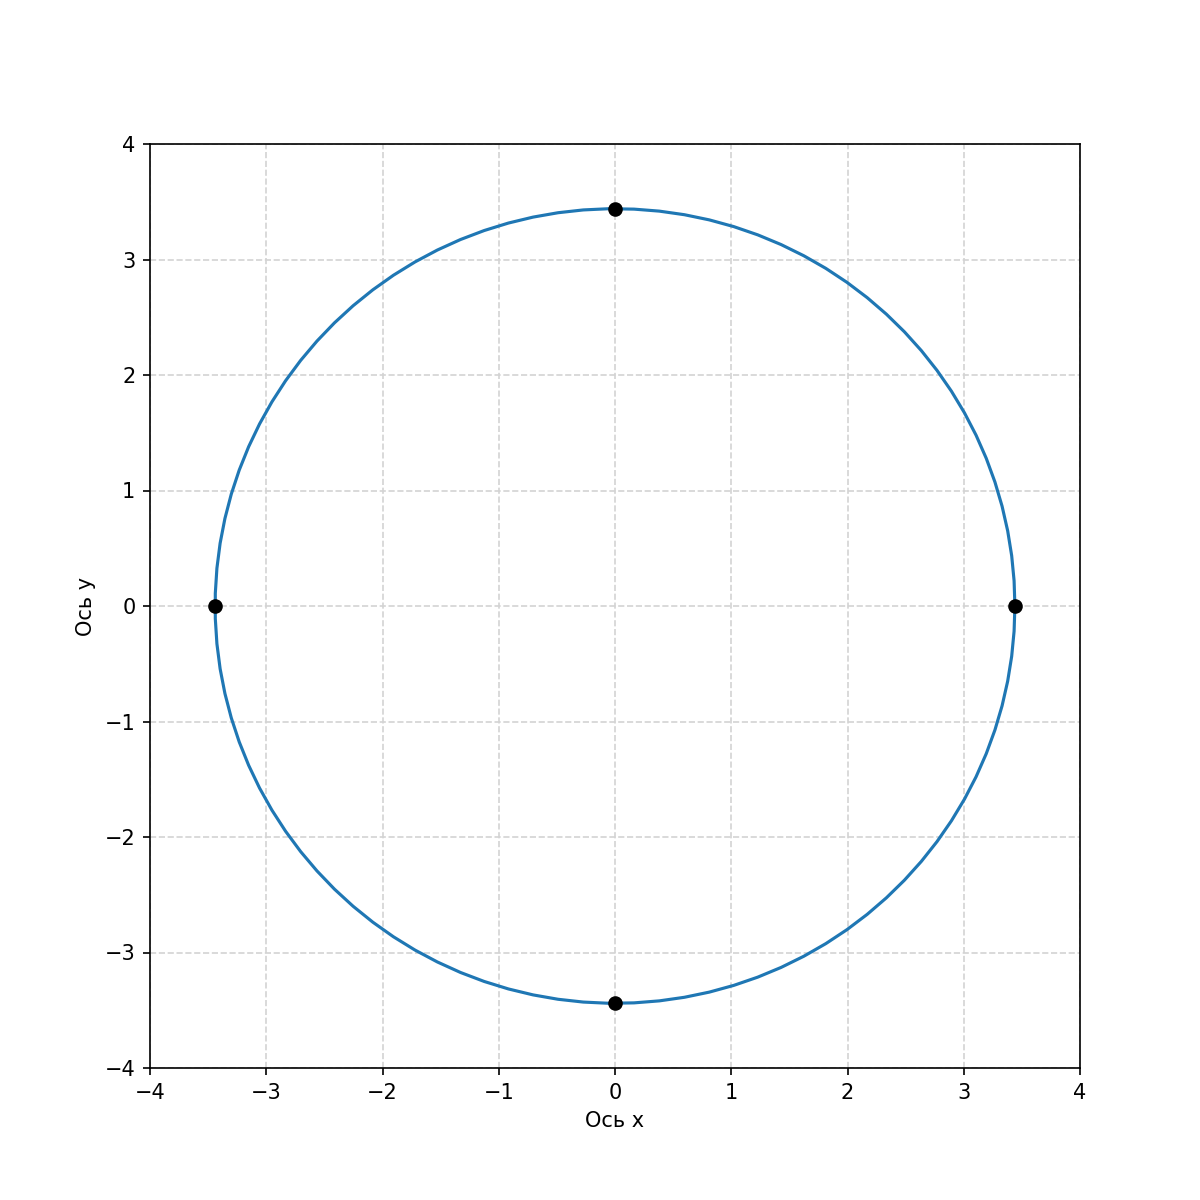
\includegraphics[width=0.5\textwidth]{Низк_цил_Oxy-1}&
        %             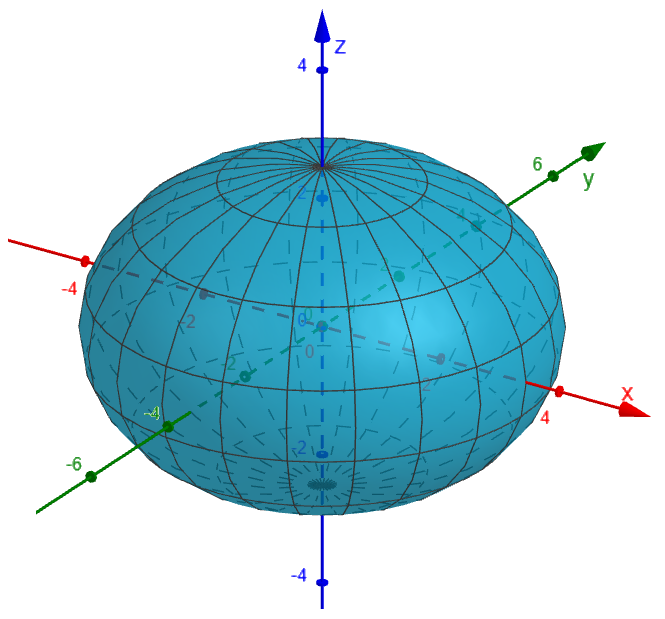
\includegraphics[width=0.5\textwidth]{Низкий_цилиндр_эллипсоид_2}\\
        %             \text{Сечение низкого цилиндра Oxy} & 
        %             \text{Эллипсоид низкого цилиндра}
        %         \end{array}$
        %     \end{center}
        % \end{figure}
        
        % \begin{figure}[h]
        %     \centering
        %     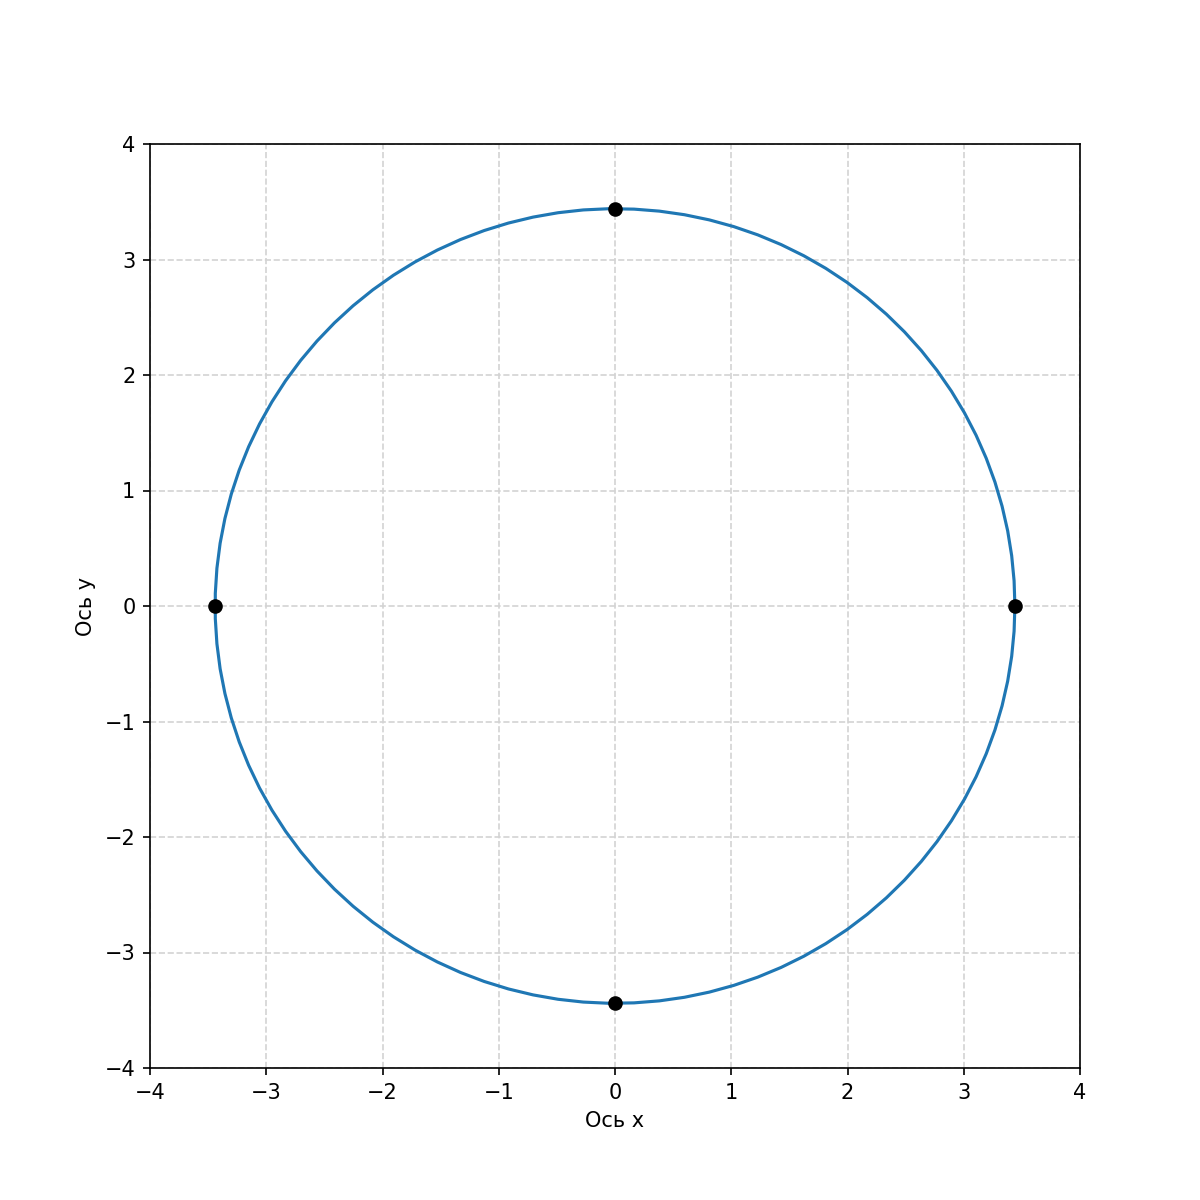
\includegraphics[width=0.8\textwidth]{Низк_цил_Oxy-1}
        % \end{figure}
        %         \begin{figure}[h]
        %     \centering
        %     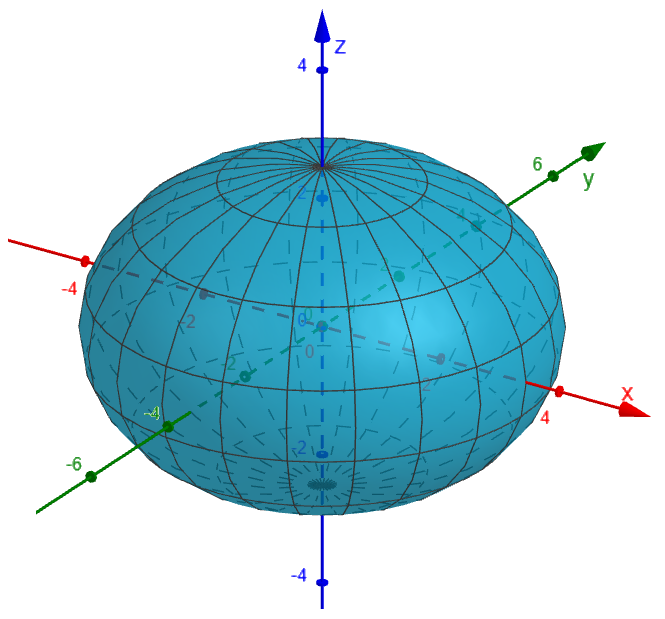
\includegraphics[width=0.8\textwidth]{Низкий_цилиндр_эллипсоид_2}
        % \end{figure}

        % \begin{figure}[h]
        %     \begin{center}$
        %         \begin{array}{cc}
        %             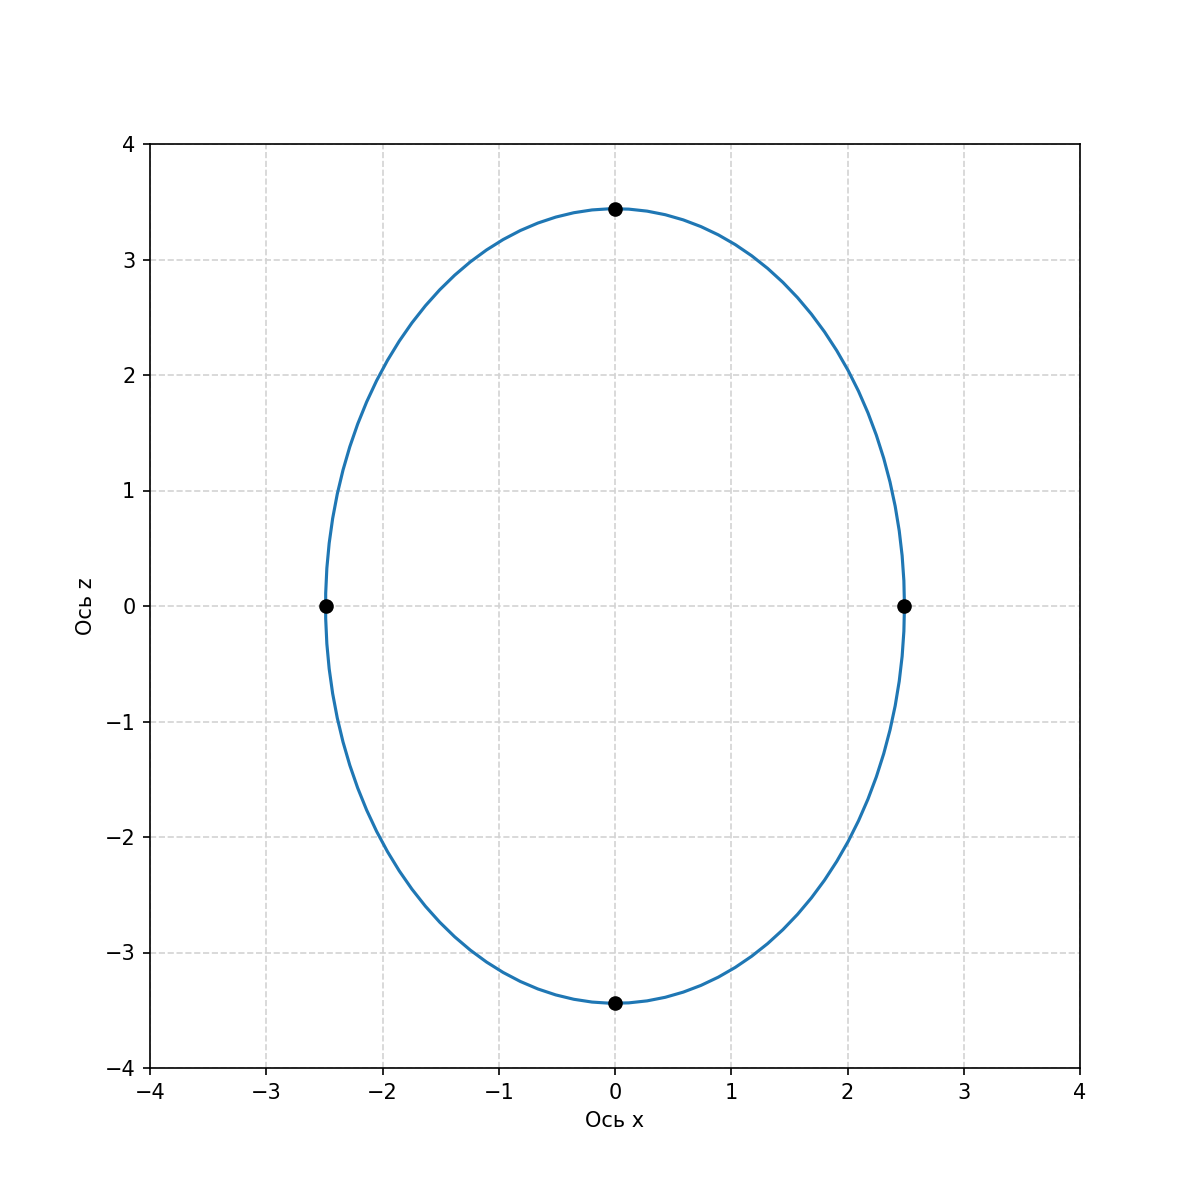
\includegraphics[width=0.5\textwidth]{Низк_цил_Oxz-1}&
        %             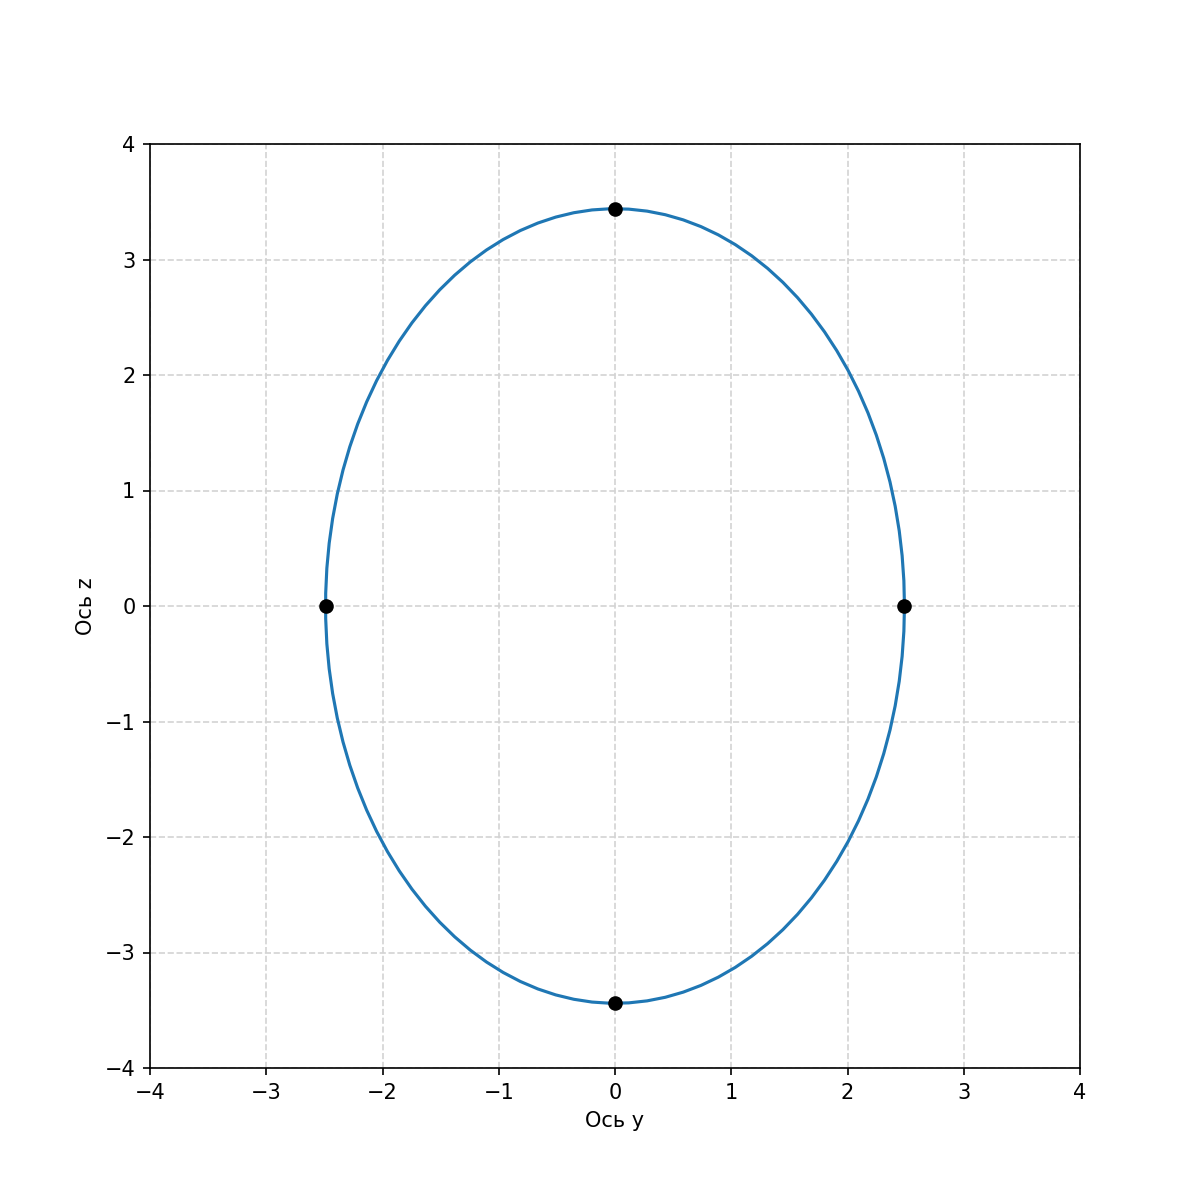
\includegraphics[width=0.5\textwidth]{Низк_цил_Oyz}\\
        %             \text{Сечение низкого цилиндра Oxz} & 
        %             \text{Сечение низкого цилиндра Oyz}
        %         \end{array}$
        %     \end{center}
        % \end{figure}

        % \begin{figure}[htb]
        % \centering
        %     \begin{subfigure}{0.5\textwidth}
        %         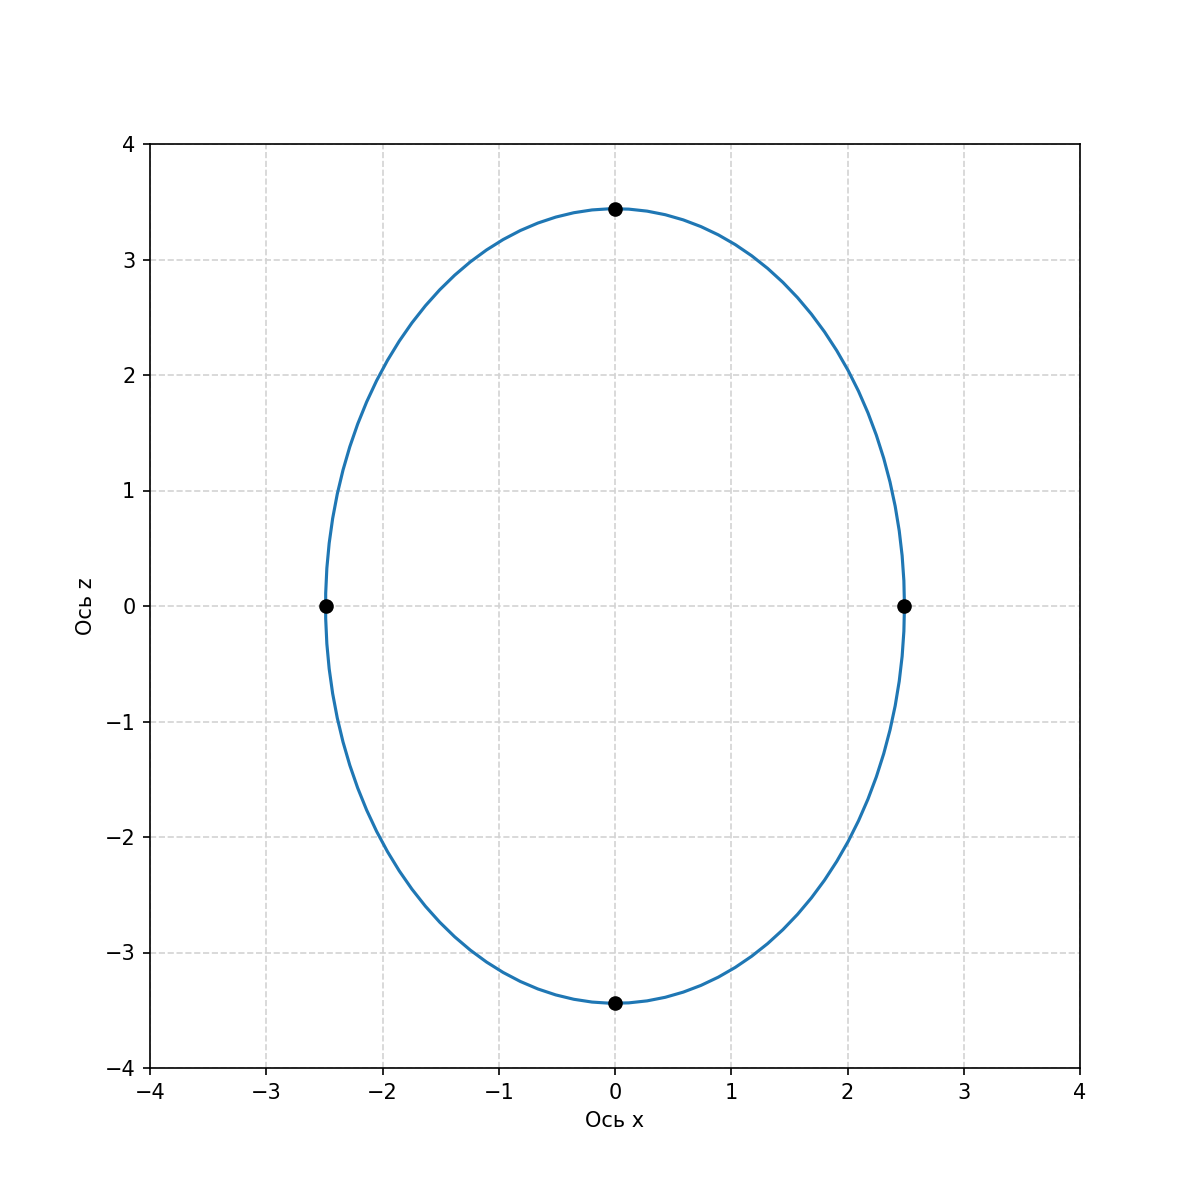
\includegraphics[width=\linewidth]{Низк_цил_Oxz-1}
        %         \caption{Сечение низкого цилиндра Oxz}
        %         % \label{fig:NET_Framework}
        %     \end{subfigure}
        
        %     \begin{subfigure}{0.5\textwidth}
        %          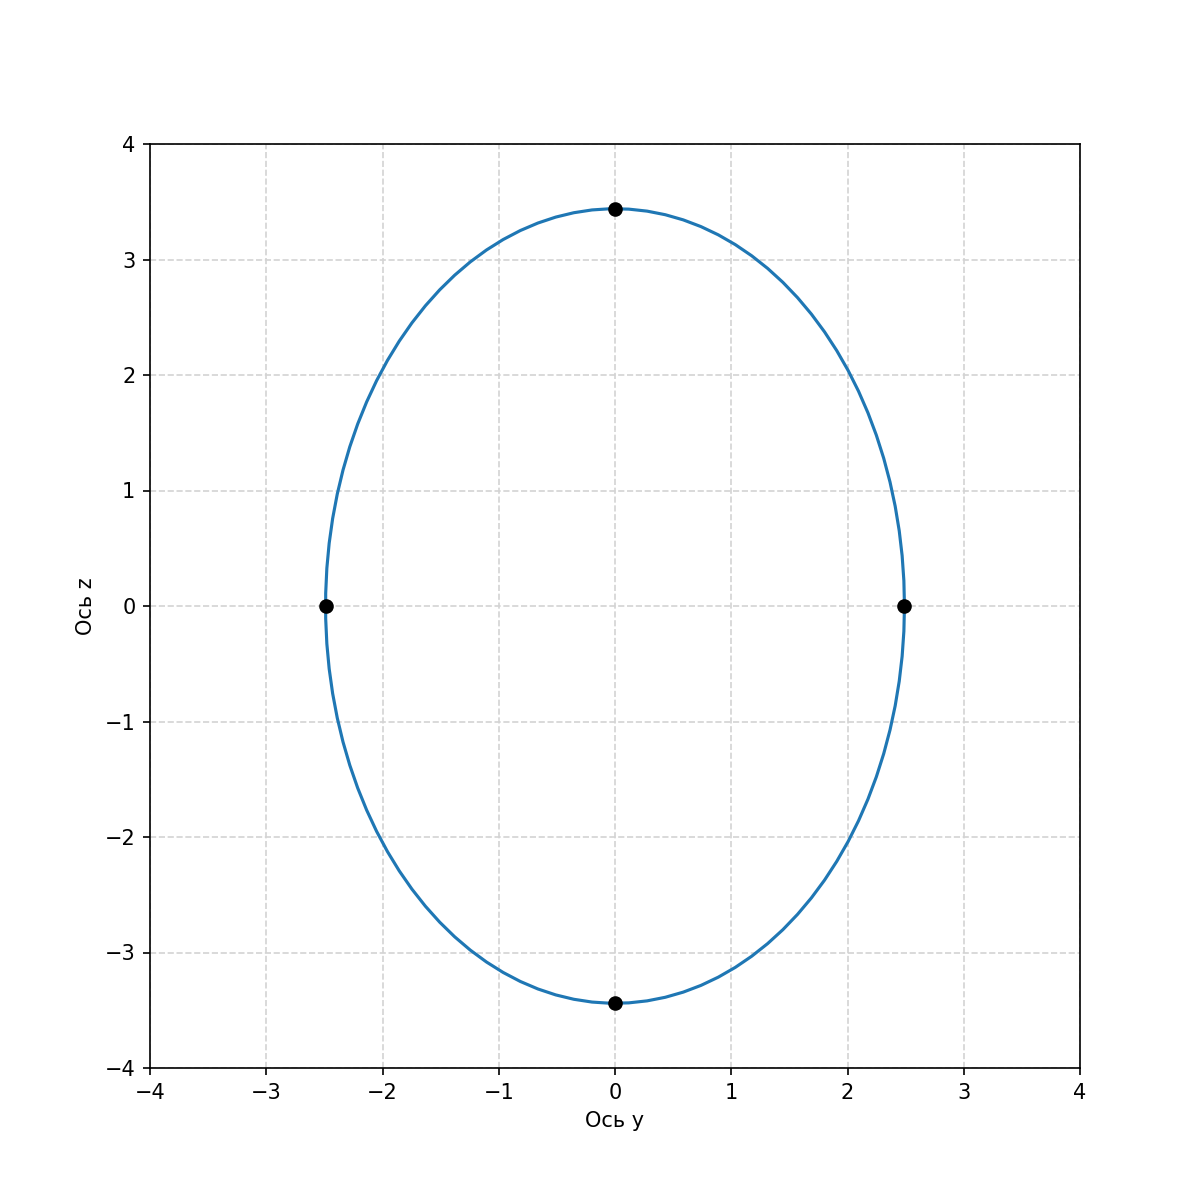
\includegraphics[width=\linewidth]{Низк_цил_Oyz}
        %         \caption{Сечение низкого цилиндра Oyz}
        %         % \label{fig:SQL_Sprache}
        %     \end{subfigure}
        % \end{figure}
    
        \begin{figure}[h]
        \centering
            \begin{subfigure}{1\textwidth}
                \begin{center}$
                    \begin{array}{cc}
                        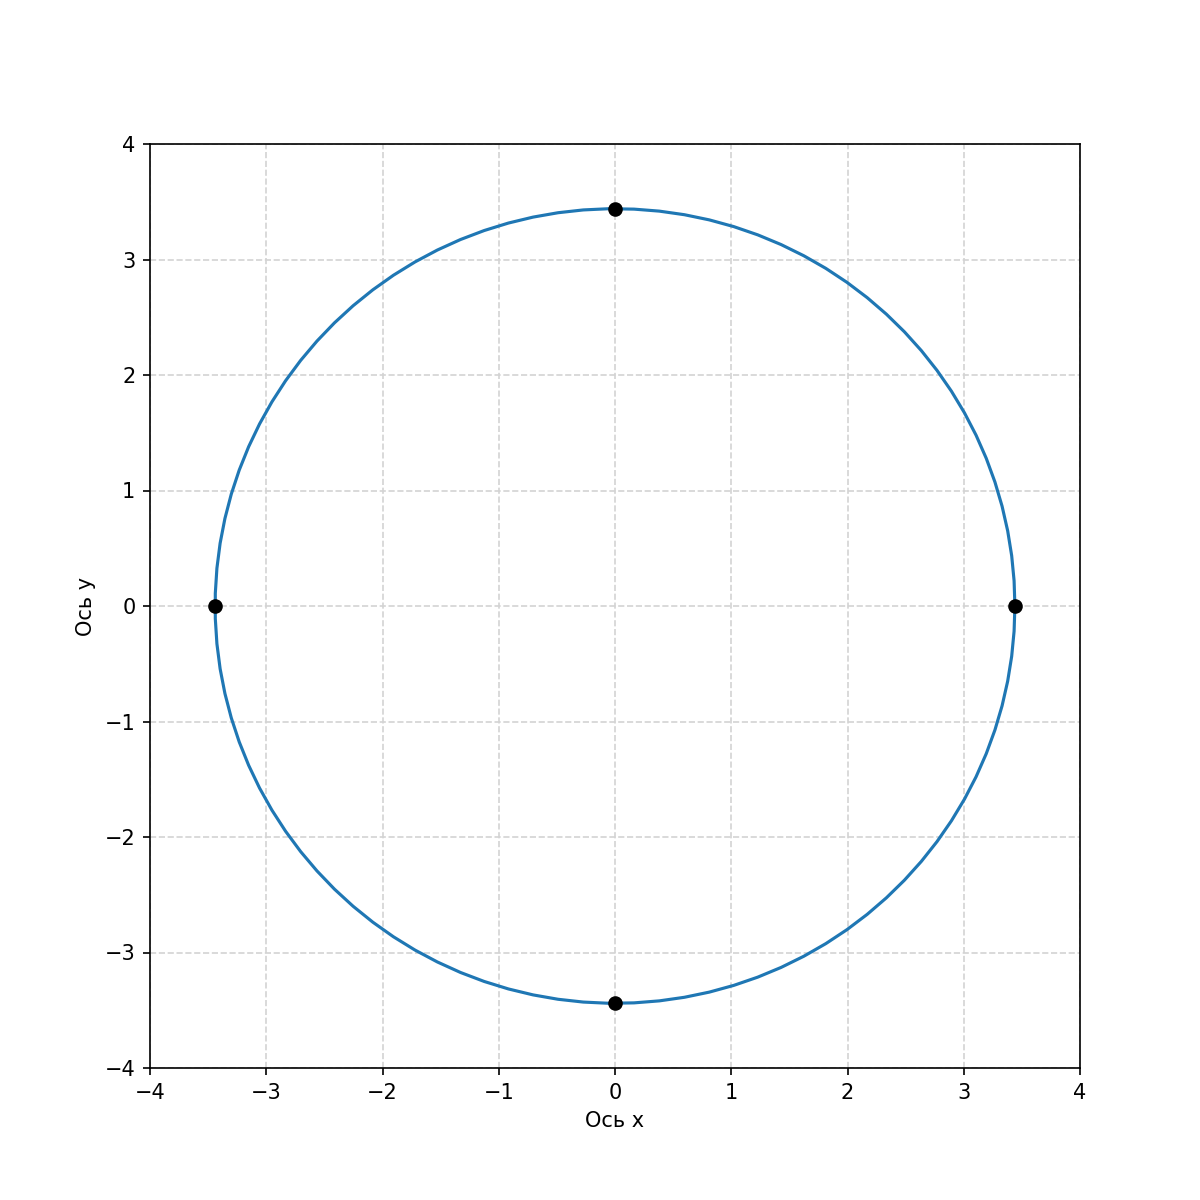
\includegraphics[width=0.5\textwidth]{Низк_цил_Oxy-1}&
                        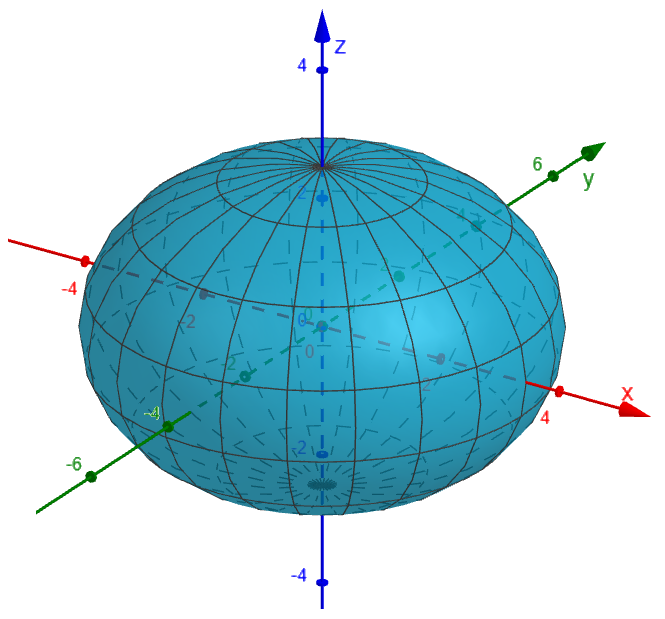
\includegraphics[width=0.5\textwidth]{Низкий_цилиндр_эллипсоид_2}\\
                        \text{Сечение низкого цилиндра Oxy.} & 
                        \text{Эллипсоид низкого цилиндра.}
                    \end{array}$
                \end{center}
            \end{subfigure}
        
            \begin{subfigure}{1\textwidth}
                 \begin{center}$
                    \begin{array}{cc}
                        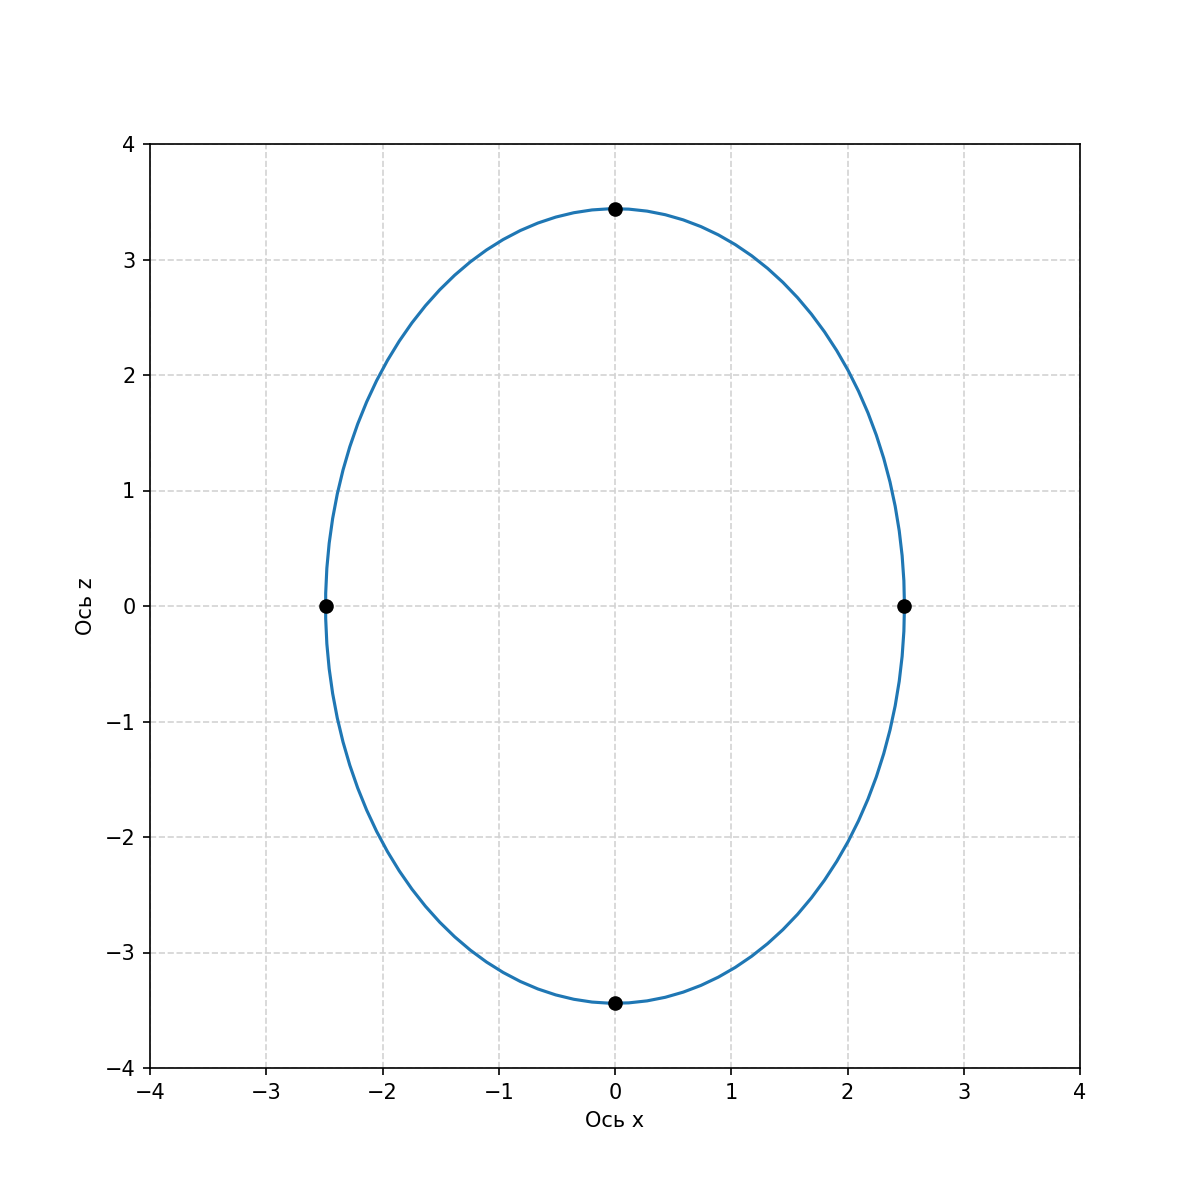
\includegraphics[width=0.5\textwidth]{Низк_цил_Oxz-1}&
                        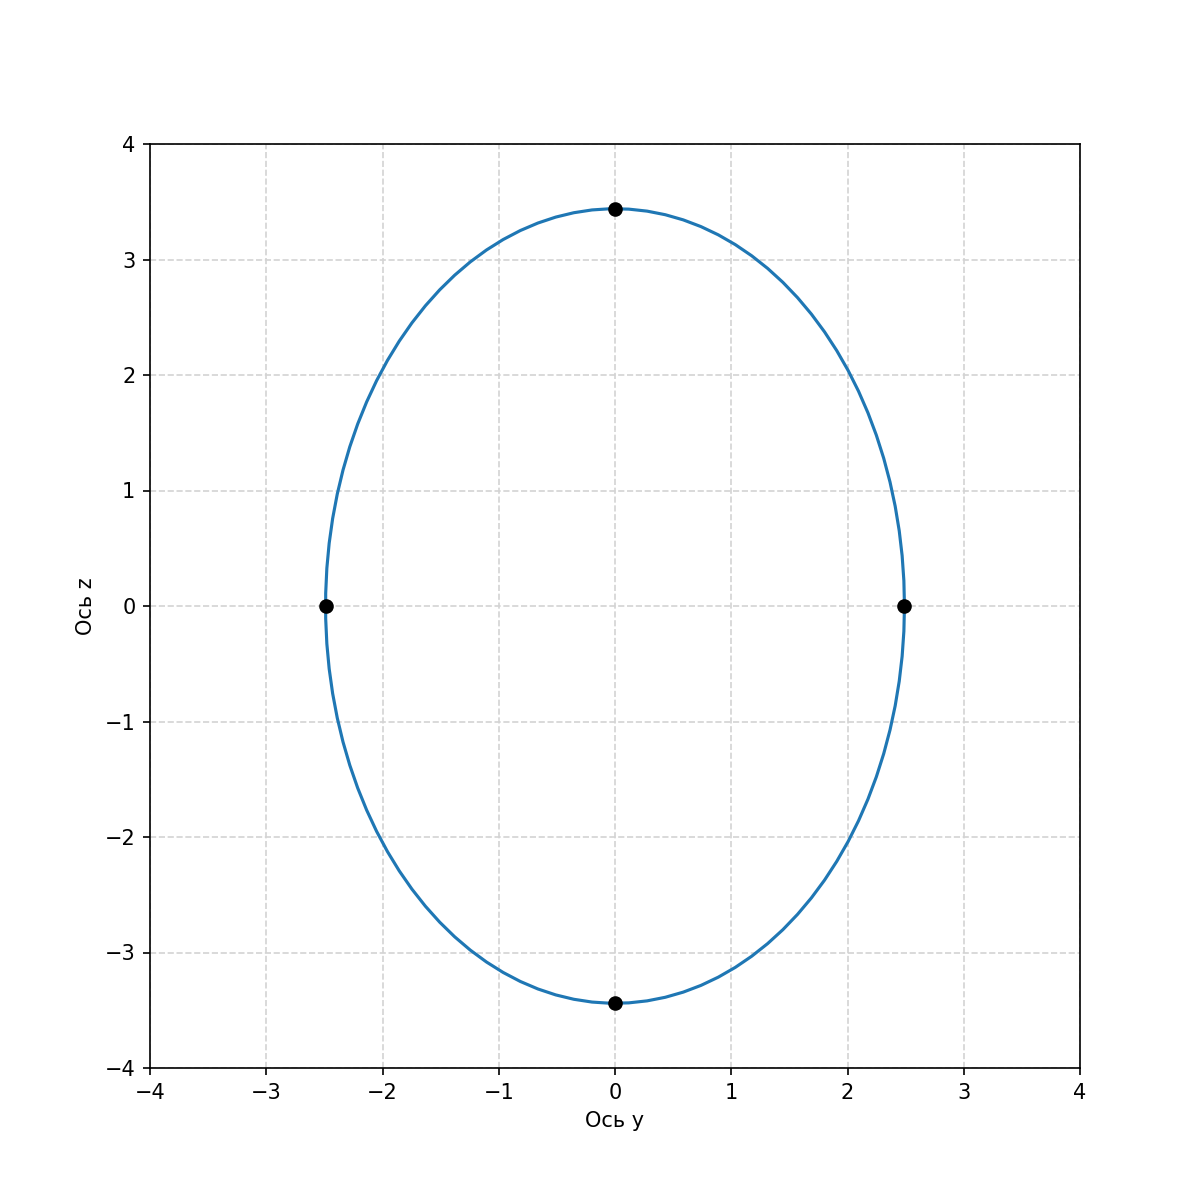
\includegraphics[width=0.5\textwidth]{Низк_цил_Oyz}\\
                        \text{Сечение низкого цилиндра Oxz.} & 
                        \text{Сечение низкого цилиндра Oyz.}
                    \end{array}$
                \end{center}
            \end{subfigure}
        \end{figure}

        \begin{figure}[h]
        \centering
            \begin{subfigure}{1\textwidth}
                \begin{center}$
                    \begin{array}{cc}
                        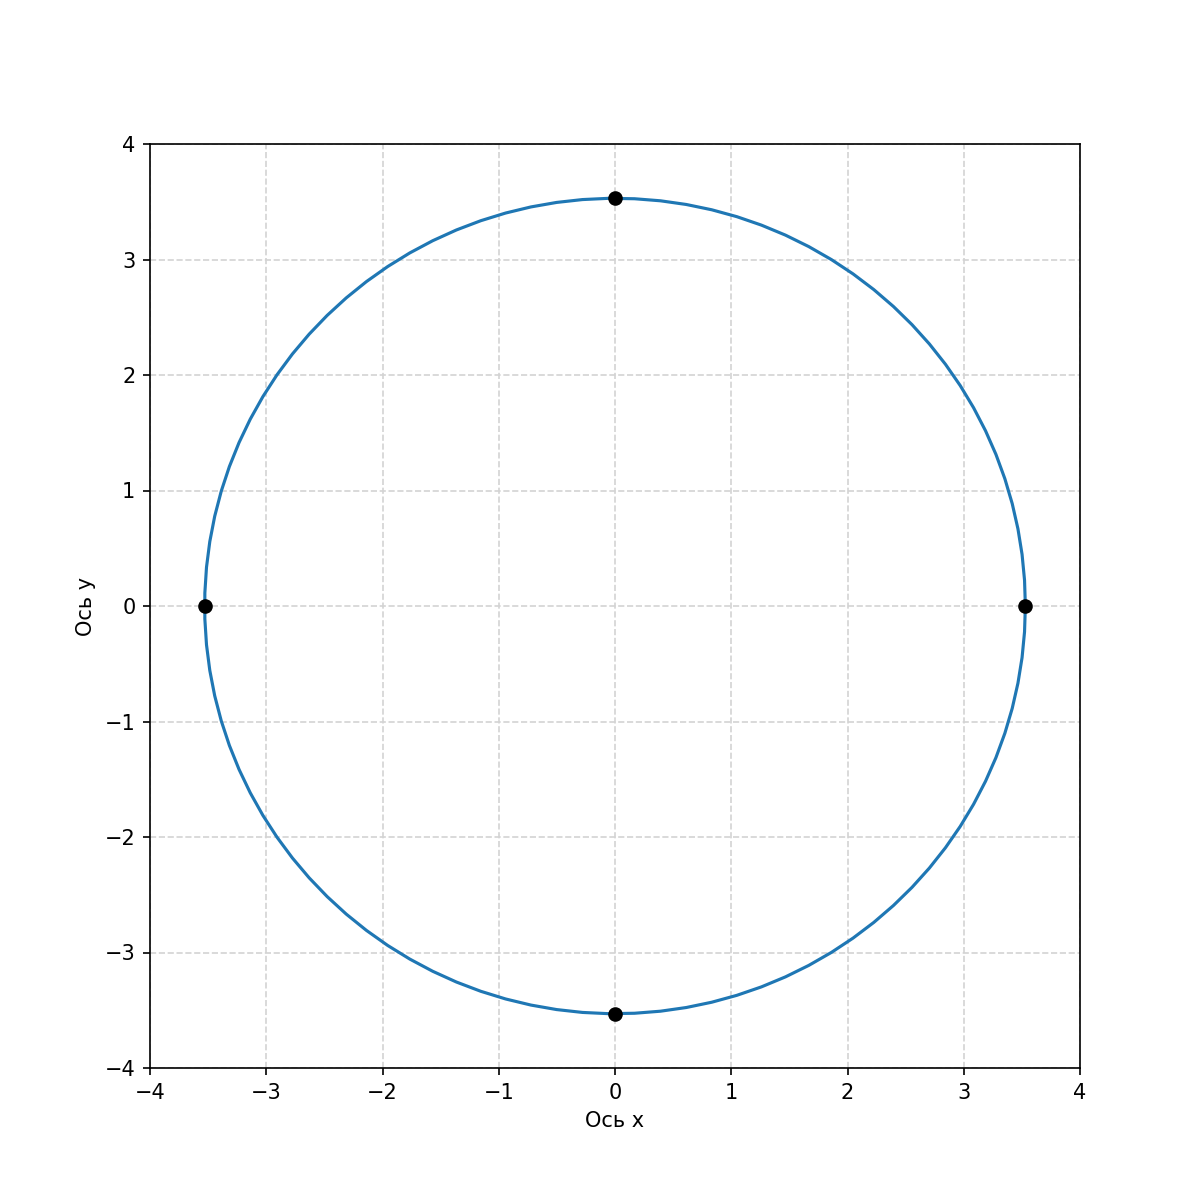
\includegraphics[width=0.5\textwidth]{Выс_цил_Oxy}&
                        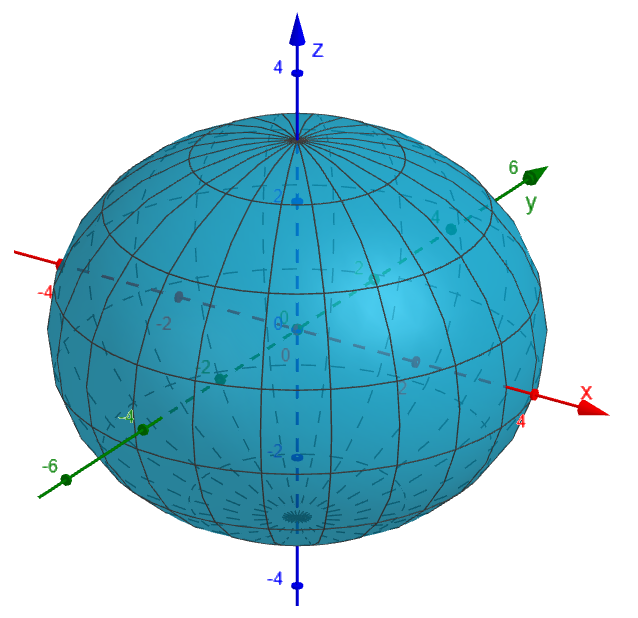
\includegraphics[width=0.5\textwidth]{Высокий_цилиндр_эллипсоид}\\
                        \text{Сечение высокого цилиндра Oxy.} & 
                        \text{Эллипсоид высокого цилиндра.}
                    \end{array}$
                \end{center}
            \end{subfigure}
        
            \begin{subfigure}{1\textwidth}
                 \begin{center}$
                    \begin{array}{cc}
                        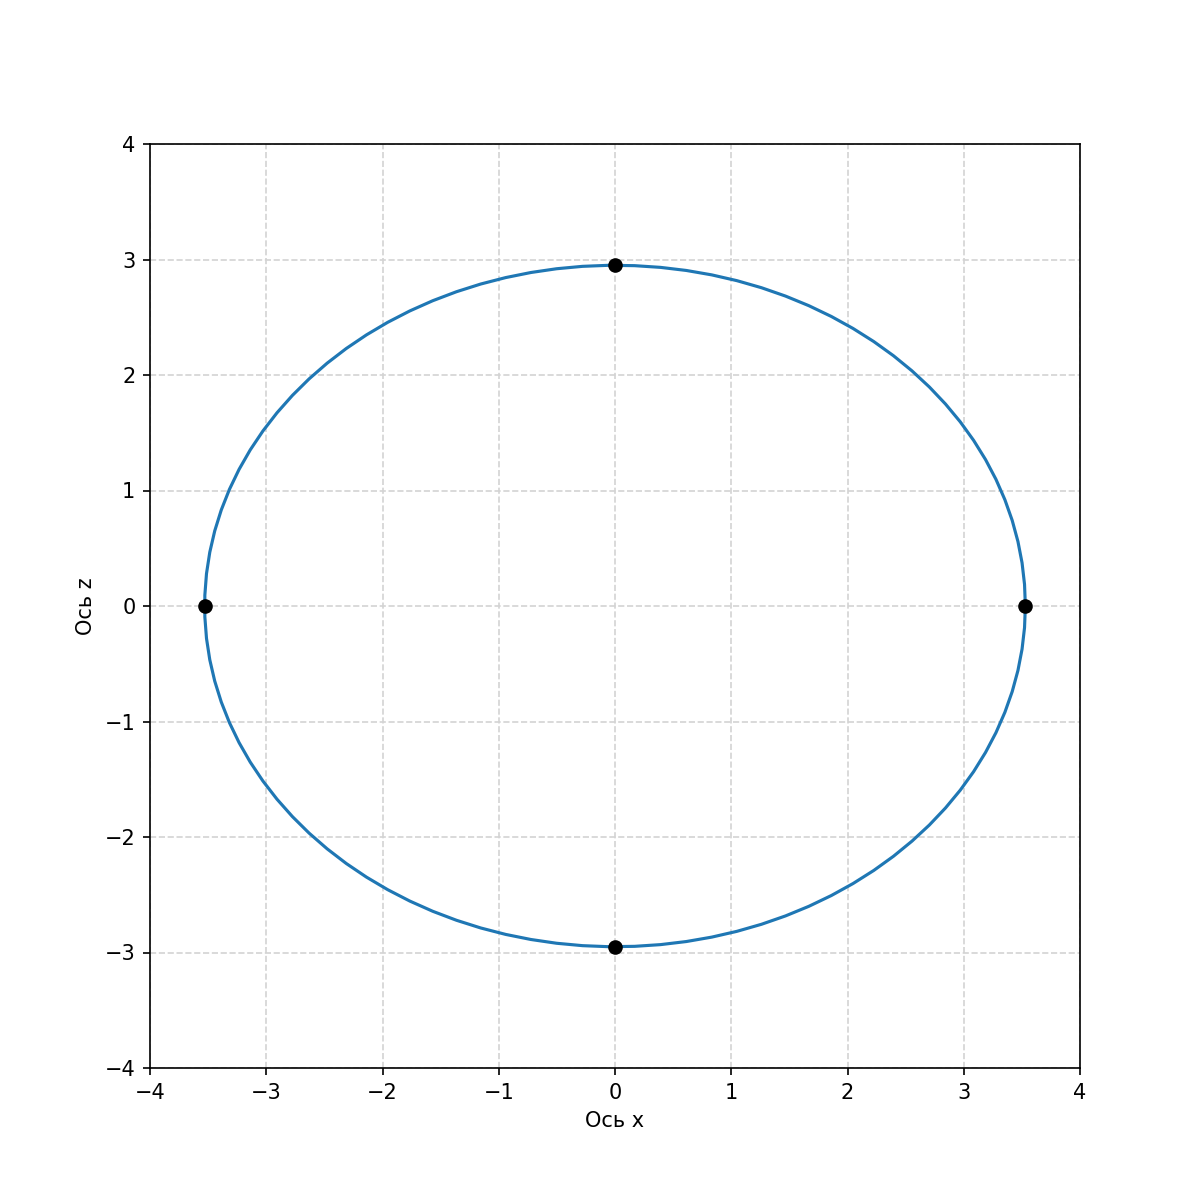
\includegraphics[width=0.5\textwidth]{Выс_цил_Oxz}&
                        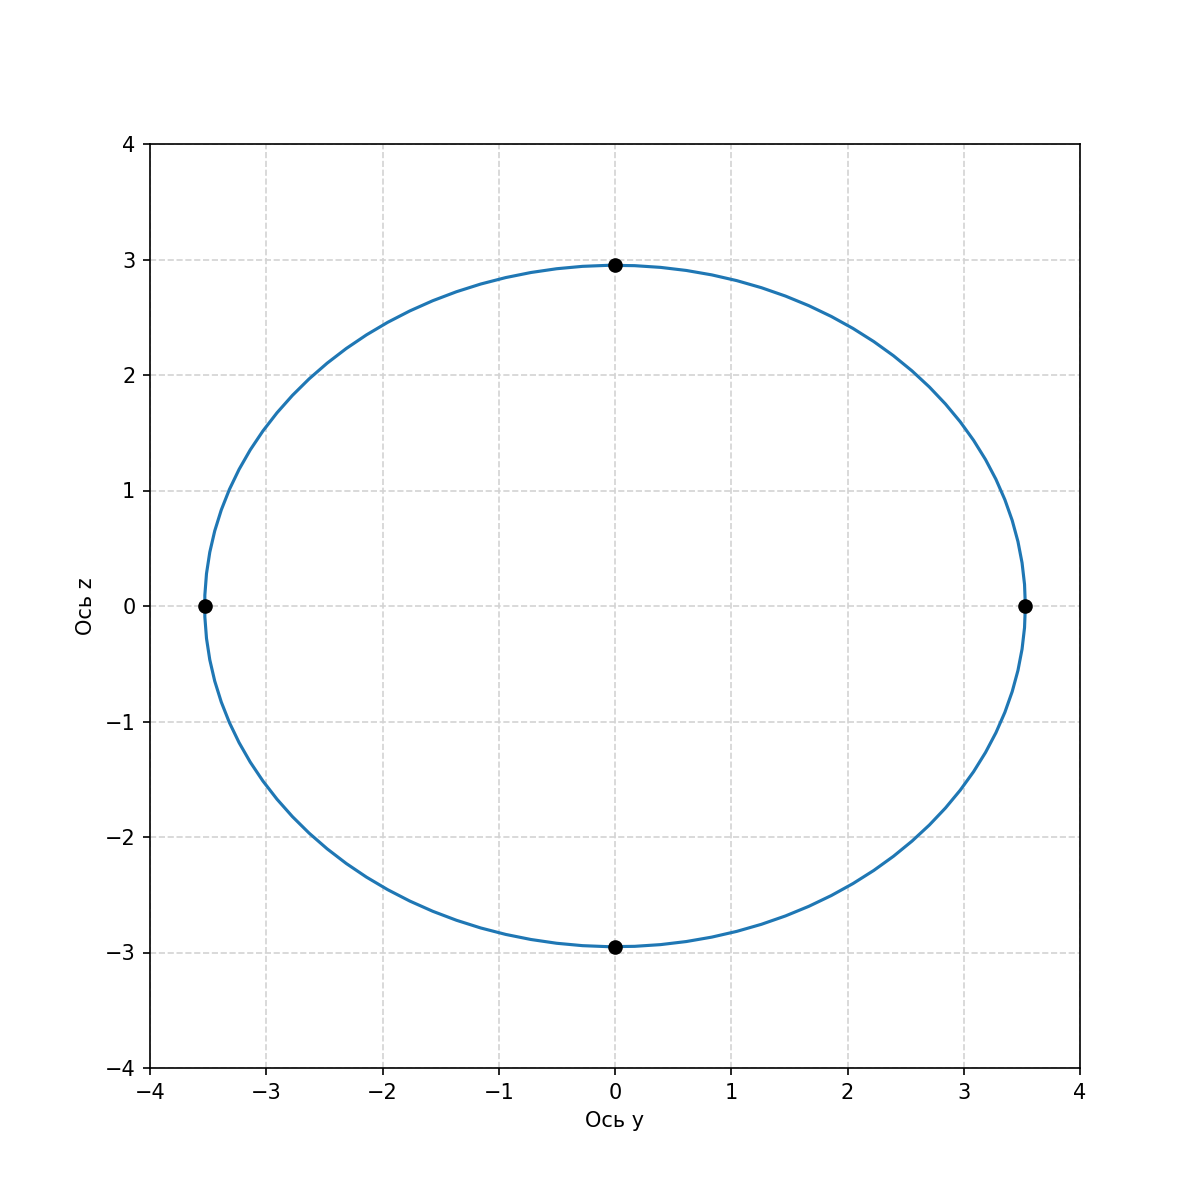
\includegraphics[width=0.5\textwidth]{Выс_цил_Oyz}\\
                        \text{Сечение высокого цилиндра Oxz.} & 
                        \text{Сечение высокого цилиндра Oyz.}
                    \end{array}$
                \end{center}
            \end{subfigure}
        \end{figure}
    
        \newpage

        \textbf{а) Эллипсоид инерции параллелепипеда.}

        Аналогично определим $r = 10/\sqrt{T^2-T_p^2}$ условных единиц.
        
        \begin{table}[h]
            \centering
            \caption{Расчет $r$ для осей параллелепипеда}
            \begin{tabular}{|c|c|c|c|c|c|c|c|}
                \hline
                Ось & $Ox$ & $Oy$ & $Oz$ &
                $MM'$ & $EE'$ & $PP'$ & $AC'$ \\ 
                \hline
                $T,\;c$ & 7,01 & 6,55 & 5,65 &
                6,52  & 5,81  & 5,97  & 6,05  \\ 
                \hline
                $1/\sqrt{T^2-T^2_p},\;1/c$ & 0,19 & 0,21 & 0,29 &
                0,21  & 0,27  & 0,25  & 0,25  \\ 
                \hline
                $r$, усл. ед. & 1,85 & 2,09 & 2,90 &
                2,11  & 2,70  & 2,53  & 2,46  \\ 
                \hline
            \end{tabular}
        \end{table}

        \begin{figure}[h]
        \centering
            \begin{subfigure}{1\textwidth}
                \begin{center}$
                    \begin{array}{cc}
                        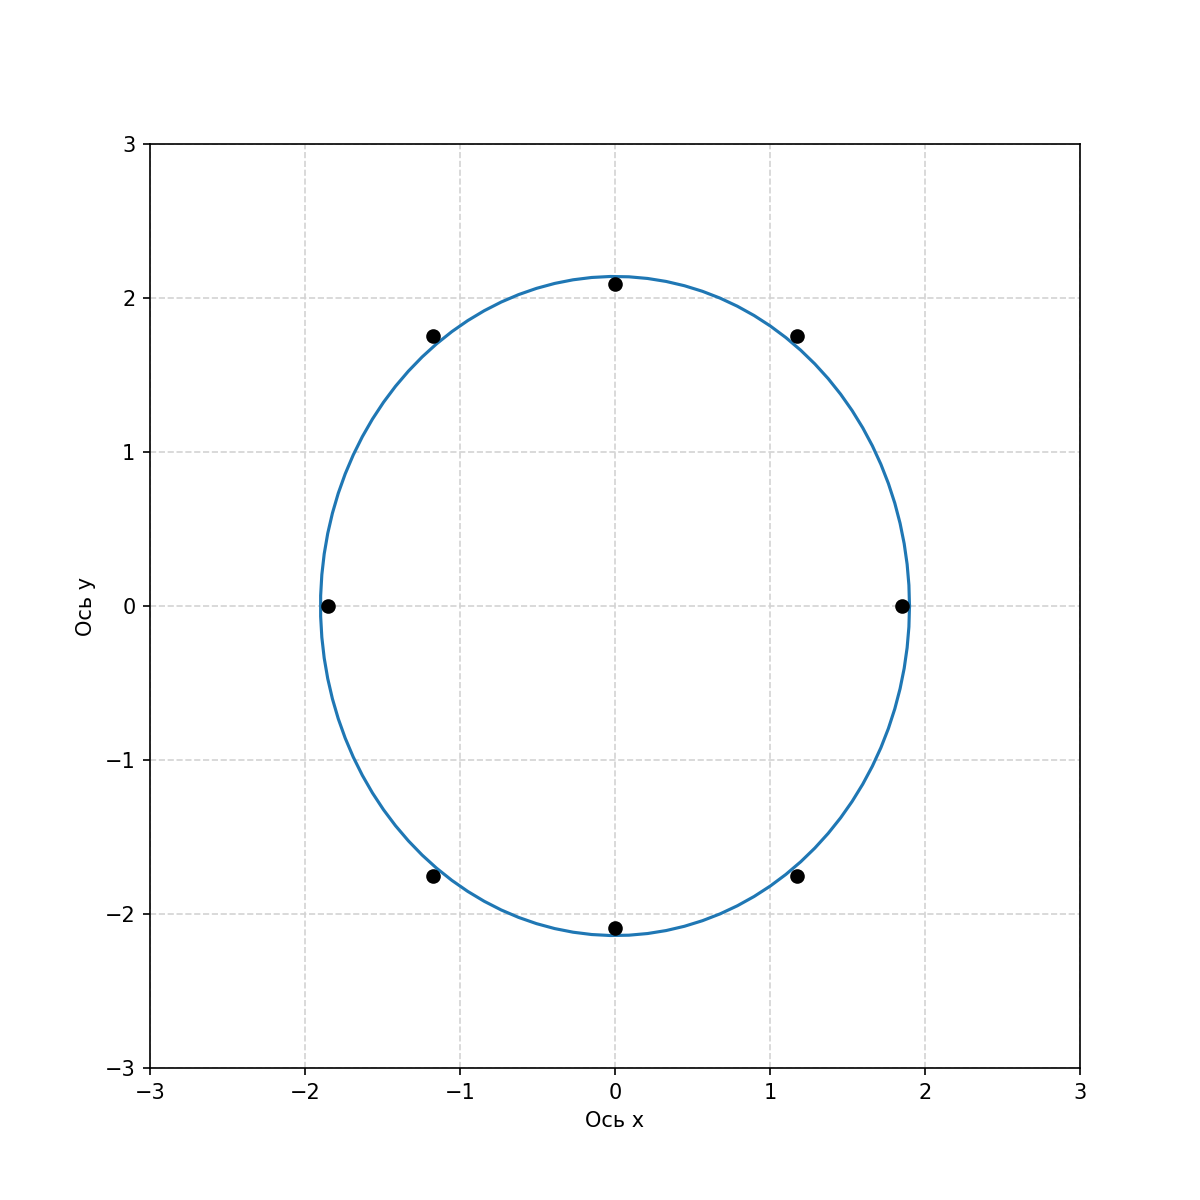
\includegraphics[width=0.5\textwidth]{Параллелепипед_Oxy-1}&
                        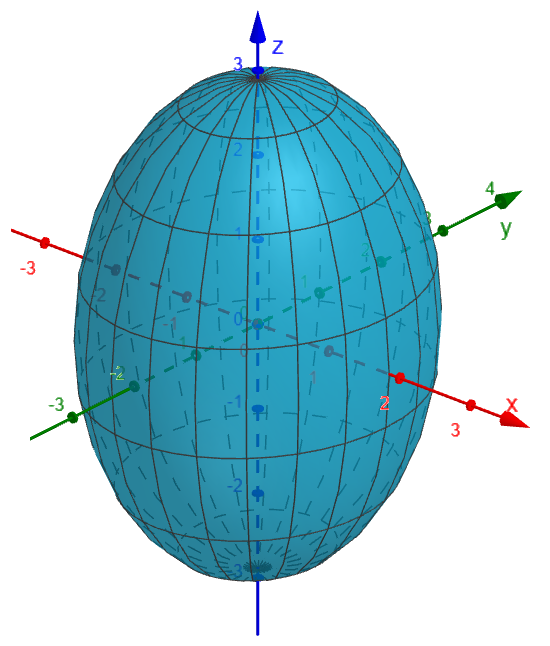
\includegraphics[width=0.5\textwidth]{Параллелепипед_эллипсоид}\\
                        \text{Сечение параллелепипеда Oxy.} & 
                        \text{Эллипсоид параллелепипеда.}
                    \end{array}$
                \end{center}
            \end{subfigure}
        
            \begin{subfigure}{1\textwidth}
                 \begin{center}$
                    \begin{array}{cc}
                        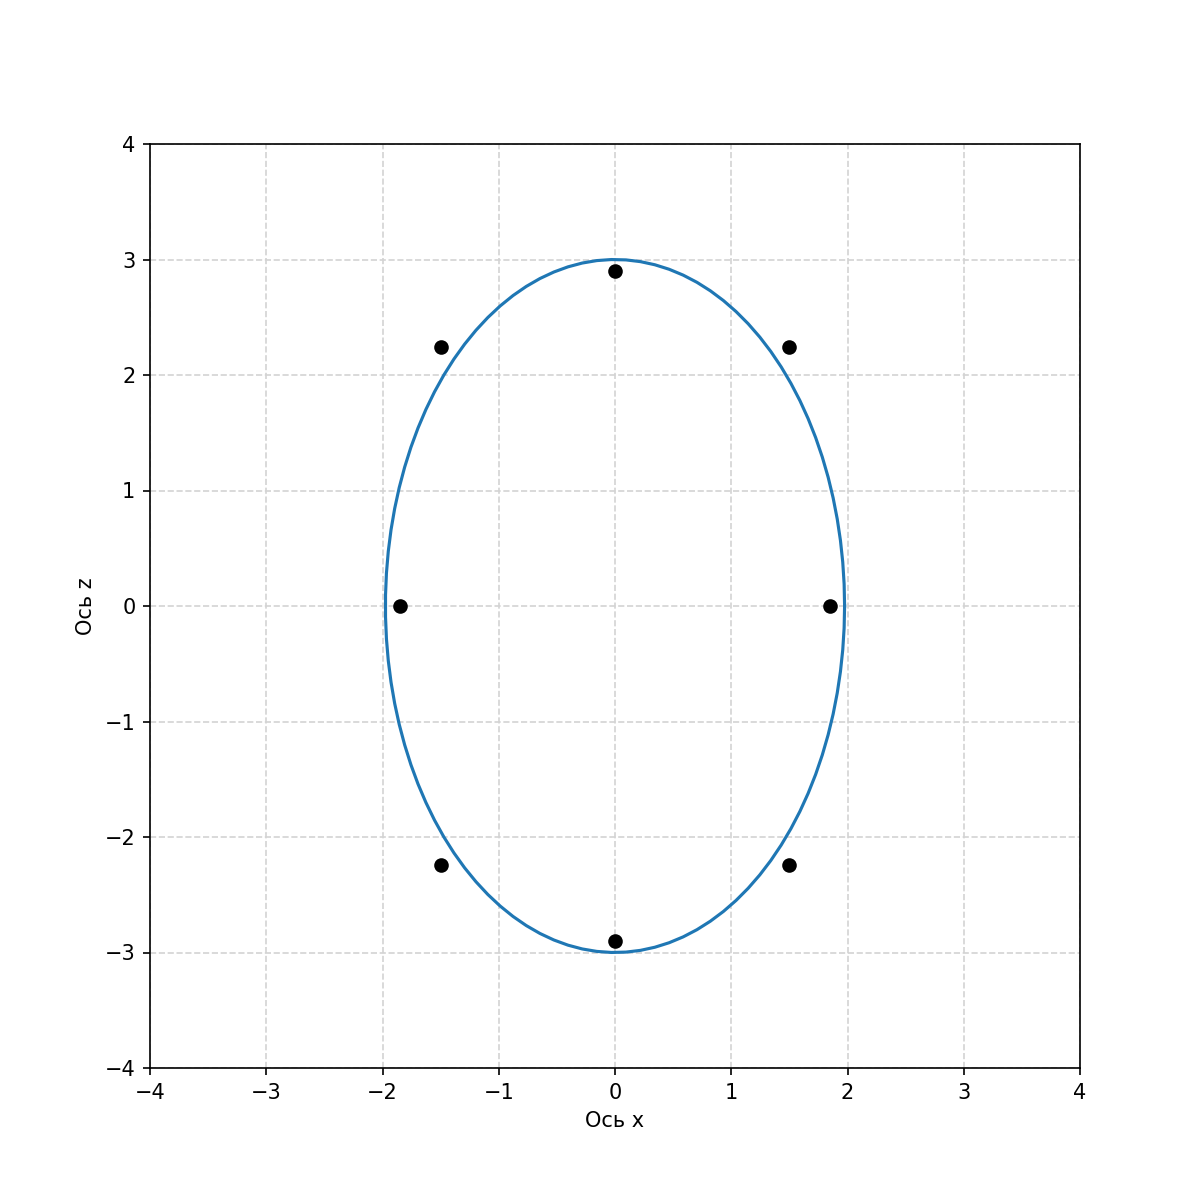
\includegraphics[width=0.5\textwidth]{Параллелепипед_Oxz}&
                        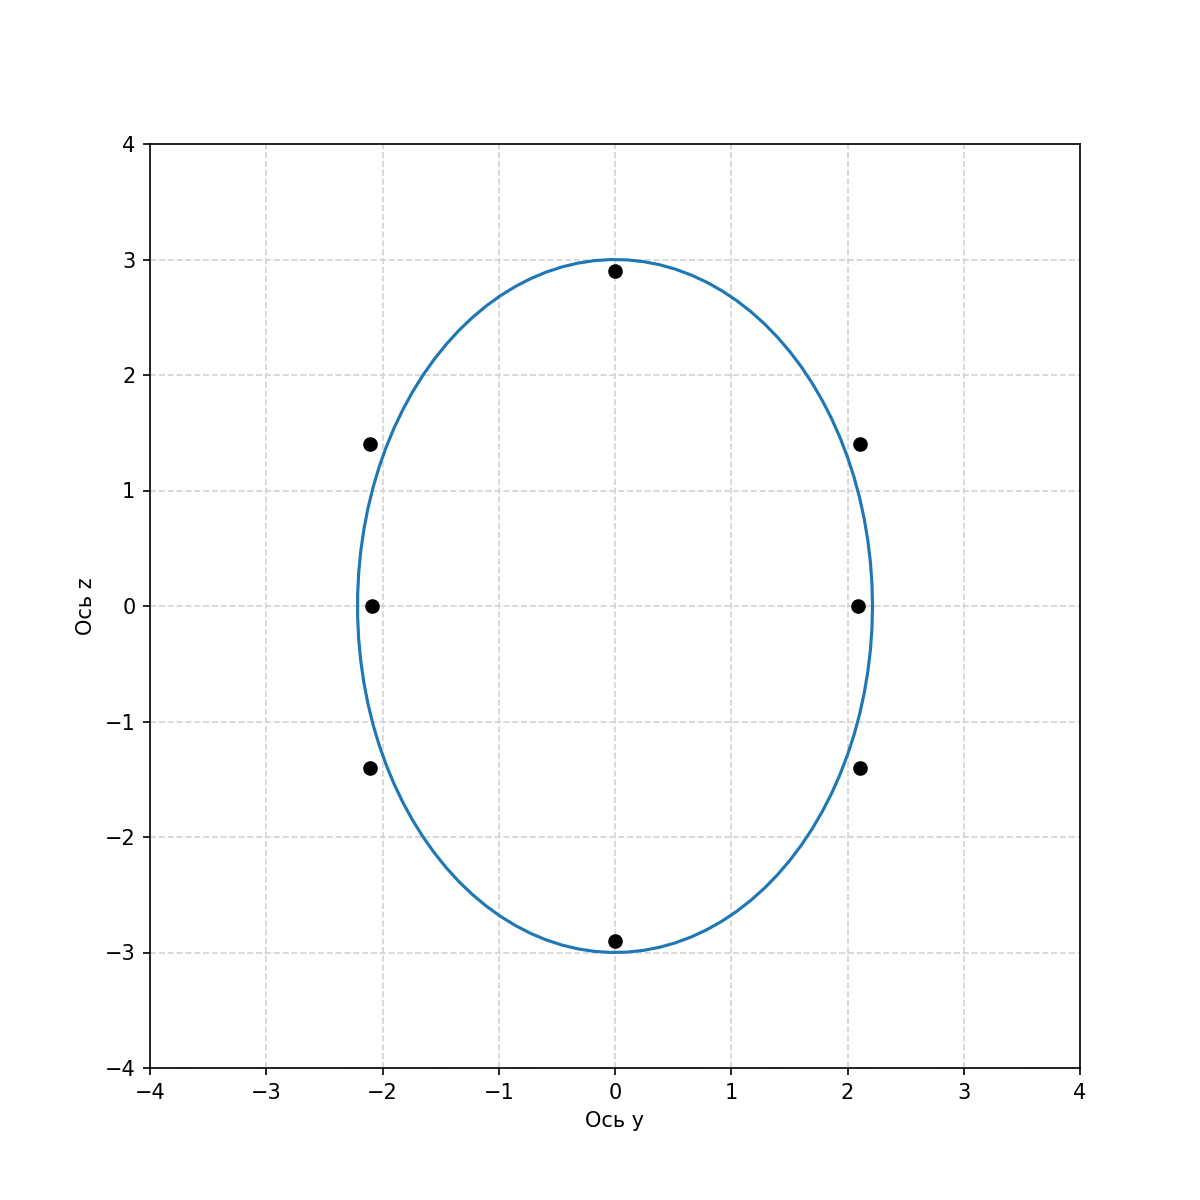
\includegraphics[width=0.5\textwidth]{Параллелепипед_Oyz}\\
                        \text{Сечение параллелепипеда Oxz.} & 
                        \text{Сечение параллелепипеда Oyz.}
                    \end{array}$
                \end{center}
            \end{subfigure}
        \end{figure}

        \textbf{а) Эллипсоид инерции куба.}

        Аналогично определим $r = 10/\sqrt{T^2-T_p^2}$ условных единиц.

        \begin{table}[h]
            \centering
            \caption{Расчет $r$ для осей куба}
            \begin{tabular}{|c|c|c|c|}
                \hline
                Ось & $X$  & $MM'$ & $AC'$ \\ 
                \hline
                $T,\;c$ & 5,35 & 5,36  & 5,37  \\ 
                \hline
                $1/\sqrt{T^2-T^2_p},\;1/c$ & 0,34 & 0,34  & 0,34  \\ 
                \hline
                $r$, усл. ед. & 3,42 & 3,41  & 3,38  \\ 
                \hline
            \end{tabular}
        \end{table}
            
        \begin{figure}[h]
        \centering
            \begin{subfigure}{1\textwidth}
                \begin{center}$
                    \begin{array}{cc}
                        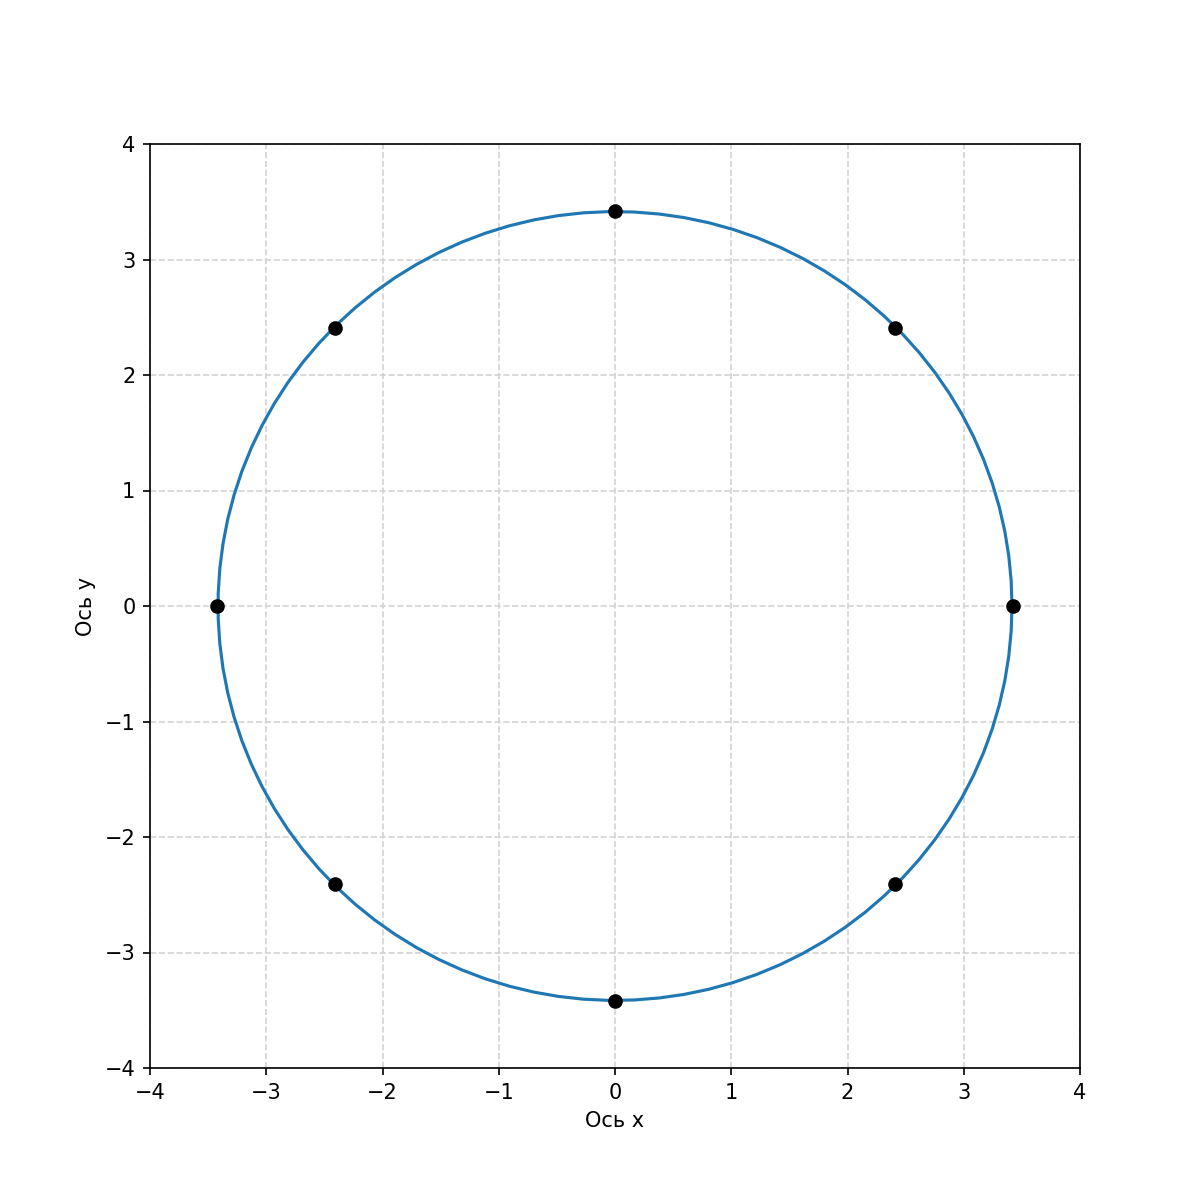
\includegraphics[width=0.5\textwidth]{Куб_Oxy}&
                        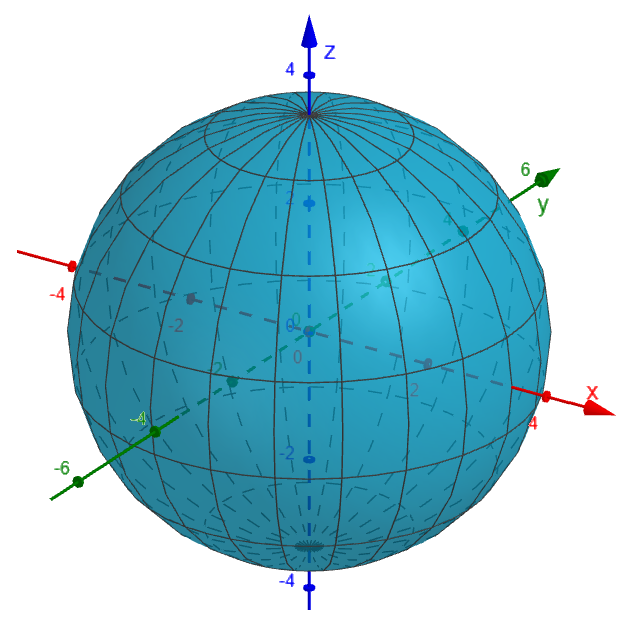
\includegraphics[width=0.5\textwidth]{Куб_эллипсоид}\\
                        \text{Сечение куба Oxy.} & 
                        \text{Эллипсоид куба.}
                    \end{array}$
                \end{center}
            \end{subfigure}
        
            \begin{subfigure}{1\textwidth}
                 \begin{center}$
                    \begin{array}{cc}
                        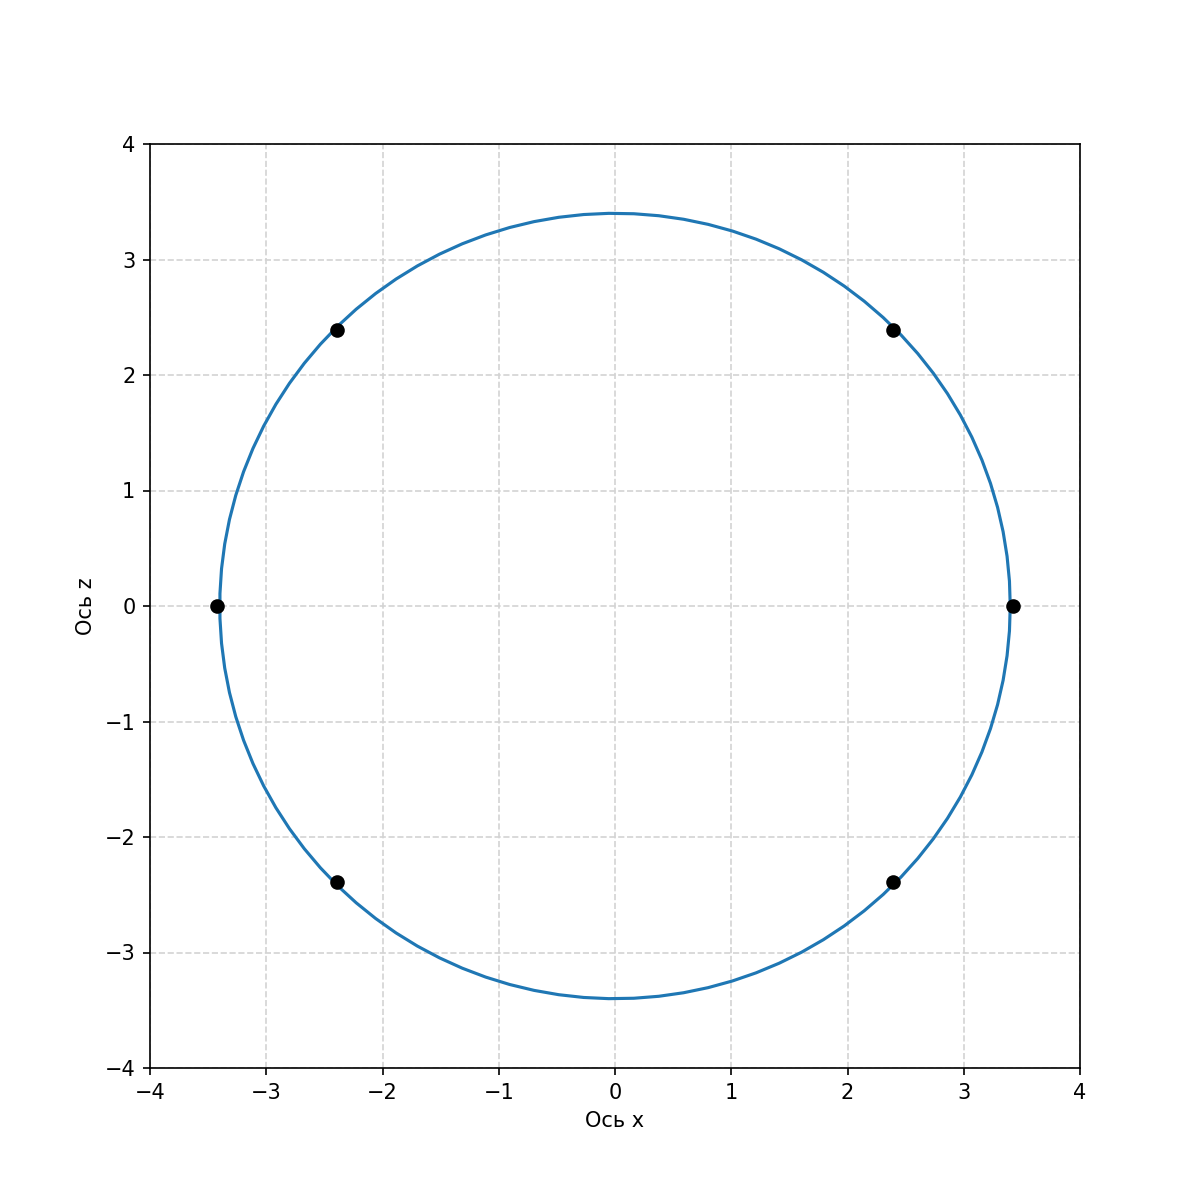
\includegraphics[width=0.5\textwidth]{Куб_Oxz}&
                        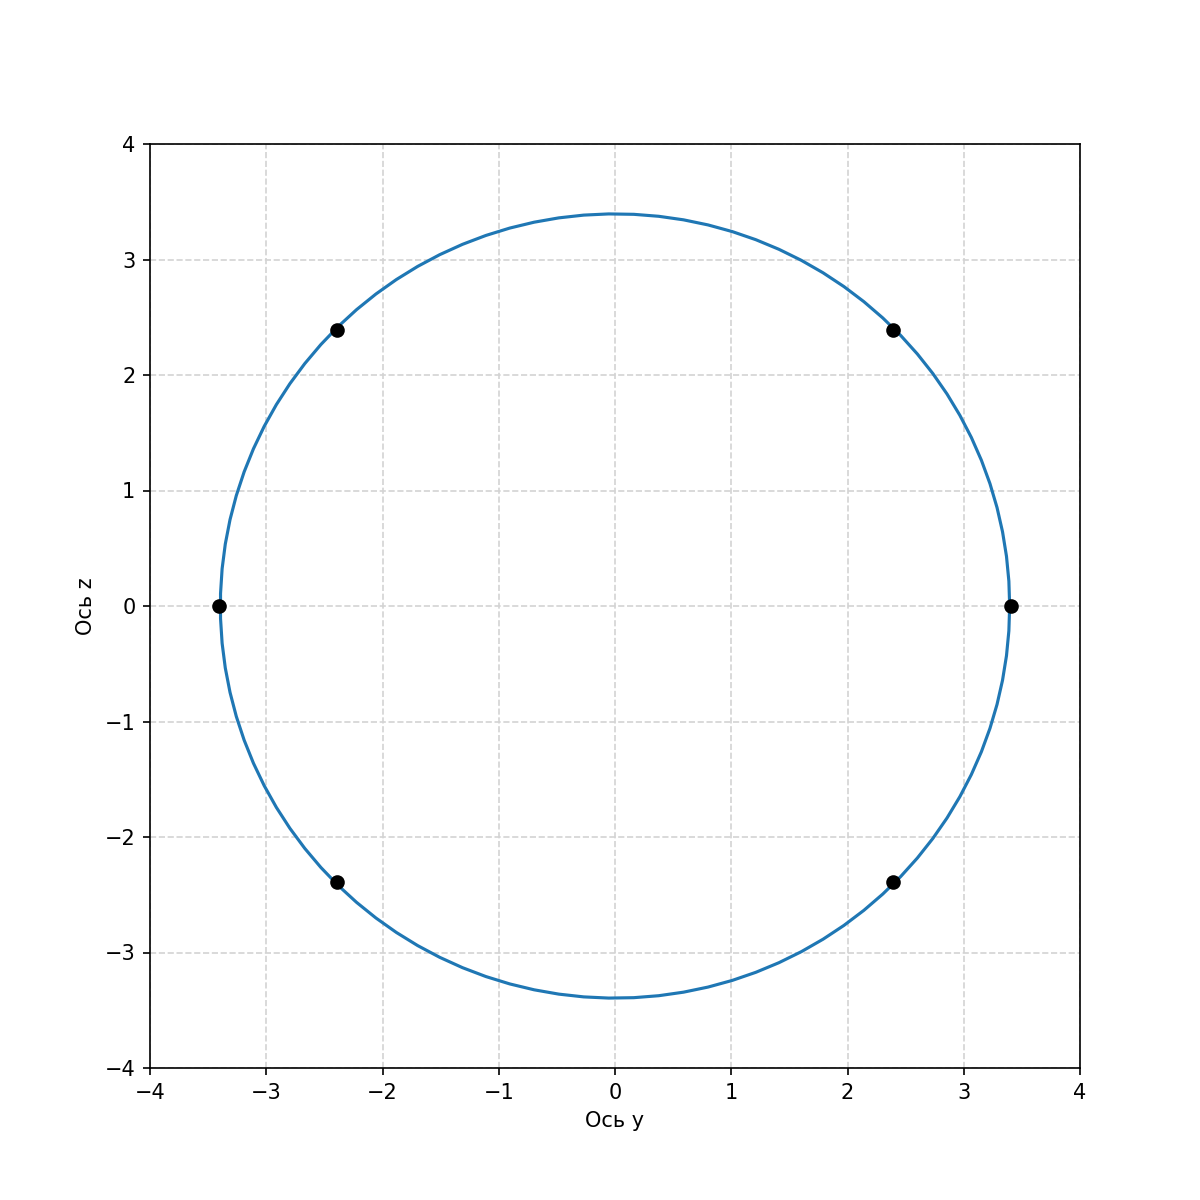
\includegraphics[width=0.5\textwidth]{Куб_Oyz}\\
                        \text{Сечение куба Oxz.} & 
                        \text{Сечение куба Oyz.}
                    \end{array}$
                \end{center}
            \end{subfigure}
        \end{figure}
        
        
        
        
        

    \section*{Обработка результатов измерений}
        7. Проверим, является ли зависимость $T^2$ от $I$ линейной. Преобразовывая формулу (4), получим:
        \begin{equation*}
            T^2 = \frac{4\pi}{f}I + \frac{4\pi}{f}I_p =
            \frac{4\pi}{f}I + T_p^2 = kI + b,
        \end{equation*}
        т.е. это линейная зависимость.
        Соберем данные для всех измеренных моментов инерции и периодов, построим график.
        
        \begin{table}[ht]
            \centering
            \caption{Периоды колебаний и моменты инерции}
            \begin{tabular}{|c|c|c|c|c|c|c|}
                \hline
                $I,\;10^{-3} кг\cdot м^2$
                & 1,549 & 1,539 & 1,554 
                & 2,191 & 2,181 & 2,534 \\ 
                \hline
                $T$, c
                & 5,3   & 5,34  & 5,36  
                & 5,62  & 5,65  & 5,81  \\ 
                \hline
                $T^2,\;c^2$
                & 28,09 & 28,52 & 28,73 
                & 31,58 & 31,92 & 33,76 \\ 
                \hline
                \hline
                $I,\;10^{-3} кг\cdot м^2$
                & 2,849 & 3,041 & 3,051 
                & 4,604 & 4,344 & 5,642 \\ 
                \hline
                $T$, c
                & 5,97  & 6,02  & 6,05  
                & 6,52  & 6,55  & 7,01  \\ 
                \hline
                $T^2,\;c^2$
                & 35,64 & 36,24 & 36,60 
                & 42,51 & 42,90 & 49,14 \\ 
                \hline
            \end{tabular}
        \end{table}

        В результате получим аппроксимирующую прямую с параметрами $k \approx 4.95\;\frac{c^2}{кг \;\cdot \; м^2},\; b \approx 21.01\; c^2$.
        
        \begin{figure}[ht]
            \begin{center}
                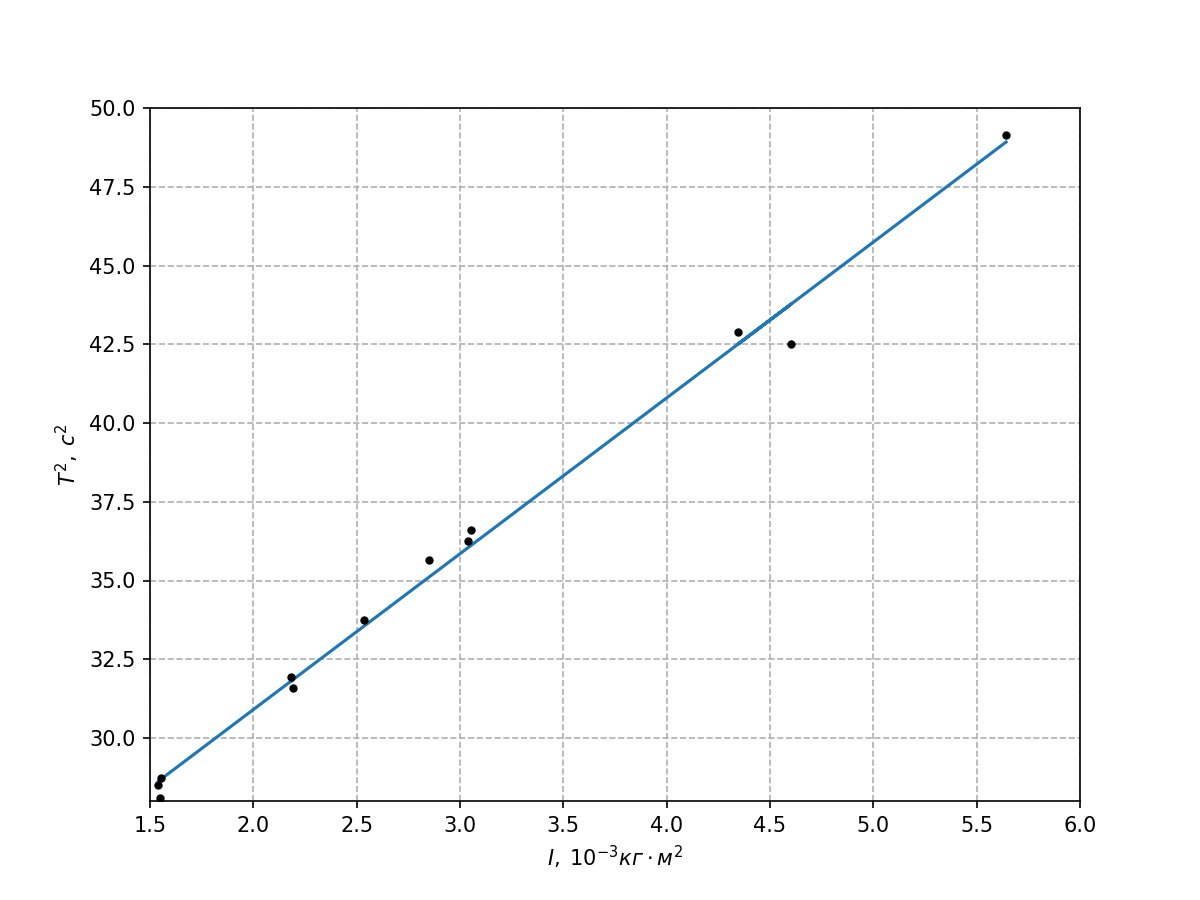
\includegraphics[width=1\textwidth]{T_2_from_I}
                \caption*{Зависимость $T^2$ от $I$.}
            \end{center}
        \end{figure}
                    
        
    \newpage
    
    \section*{Вывод}
        В ходе работы были измерены периоды колебаний различных однородных тел относительно различных осей, проходящий через центр масс рассматриваемых тел.
        
        Была поддтверждена теоретическая зависимость между периодами крутильных колебаний тела относительно 
        различных осей.
        
        Были установлены положения главных осей тел и вычислены моменты инерции относительно этих осей, построены эллипсоиды инерции и из сечения на плоскости $Oxy,\;Oxz\;и\;Oyz$.

        Из графиков сечений эллипсоидов можно заметить, что точки не идеально ложатся на построенную кривую. Это обсуловленно прогрешностью, связанной со скоростью реакции человека, и пренебрегаемыми явлениями (малое затухание колебаний, провисание или необратимая деформация проволоки). Таким образом, данная установка дает заметную погрешность. Однако ее точности достаточно, чтобы определить форму графиков (прийти к тому, что это эллипсоиды) и сделать необходимые выводы. 
        
        Поскольку точки ложатся на эллипсы, выведенные теоретические формулы справедливы.

\end{document}